%% History:
% Pavel Tvrdik (26.12.2004)
%  + initial version for PhD Report
%
% Daniel Sykora (27.01.2005)
%
% Michal Valenta (3.12.2008)
% rada zmen ve formatovani (diky M. Duškovi, J. Holubovi a J. Žďárkovi)
% sjednoceni zdrojoveho kodu pro anglickou, ceskou, bakalarskou a diplomovou praci

% One-page layout: (proof-)reading on display
%%%% \documentclass[11pt,oneside,a4paper]{book}
% Two-page layout: final printing
\documentclass[11pt,twoside,a4paper]{book}   

\usepackage{wrapfig, floatrow, amsmath, url, graphicx, array}

\usepackage[czech, english]{babel}
\usepackage[T1]{fontenc} % pouzije EC fonty 
% pripadne pisete-li cesky, pak lze zkusit take:
% \usepackage[OT1]{fontenc} 
\usepackage[utf8]{inputenc}
%=-=-=-=-=-=-=-=-=-=-=-=--=%
% In case of problems with PDF fonts, one may try to uncomment this line:
%\usepackage{lmodern}
%=-=-=-=-=-=-=-=-=-=-=-=--=%
%=-=-=-=-=-=-=-=-=-=-=-=--=%
% Depending on your particular TeX distribution and version of conversion tools 
% (dvips/dvipdf/ps2pdf), some (advanced | desperate) users may prefer to use 
% different settings.
% Please uncomment the following style and use your CSLaTeX (cslatex/pdfcslatex) 
% to process your work. Note however, this file is in UTF-8 and a conversion to 
% your native encoding may be required. Some settings below depend on babel 
% macros and should also be modified. See \selectlanguage \iflanguage.
%\usepackage{czech}  %%%%%\usepackage[T1]{czech} %%%%[IL2] [T1] [OT1]
%=-=-=-=-=-=-=-=-=-=-=-=--=%

%%%%%%%%%%%%%%%%%%%%%%%%%%%%%%%%%%%%%%%
% Styles required in your work follow %
%%%%%%%%%%%%%%%%%%%%%%%%%%%%%%%%%%%%%%%
\usepackage{graphicx}
\usepackage{indentfirst} %1. odstavec jako v cestine.
\usepackage{listings}
\usepackage{color}
\usepackage{soul}
\setul{0.1ex}{}

\renewcommand{\lstlistingname}{Ukázka}

\definecolor{mygreen}{rgb}{0,0.6,0}
\definecolor{mygray}{rgb}{0.5,0.5,0.5}
\definecolor{mymauve}{rgb}{0.58,0,0.82}

\lstset{ %
  backgroundcolor=\color{white},   % choose the background color; you must add \usepackage{color} or \usepackage{xcolor}
  basicstyle=\footnotesize,        % the size of the fonts that are used for the code
  breakatwhitespace=false,         % sets if automatic breaks should only happen at whitespace
  breaklines=true,                 % sets automatic line breaking
  captionpos=b,                    % sets the caption-position to bottom
  commentstyle=\color{mygreen},    % comment style
  deletekeywords={...},            % if you want to delete keywords from the given language
  escapeinside={\%*}{*)},          % if you want to add LaTeX within your code
  extendedchars=true,              % lets you use non-ASCII characters; for 8-bits encodings only, does not work with UTF-8
  frame=single,                    % adds a frame around the code
  keepspaces=true,                 % keeps spaces in text, useful for keeping indentation of code (possibly needs columns=flexible)
  keywordstyle=\color{blue},       % keyword style
  language=Octave,                 % the language of the code
  morekeywords={*,...},            % if you want to add more keywords to the set
  numbers=left,                    % where to put the line-numbers; possible values are (none, left, right)
  numbersep=5pt,                   % how far the line-numbers are from the code
  numberstyle=\tiny\color{mygray}, % the style that is used for the line-numbers
  rulecolor=\color{black},         % if not set, the frame-color may be changed on line-breaks within not-black text (e.g. comments (green here))
  showspaces=false,                % show spaces everywhere adding particular underscores; it overrides 'showstringspaces'
  showstringspaces=false,          % underline spaces within strings only
  showtabs=false,                  % show tabs within strings adding particular underscores
  stepnumber=1,                    % the step between two line-numbers. If it's 1, each line will be numbered
  stringstyle=\color{mymauve},     % string literal style
  tabsize=2,                       % sets default tabsize to 2 spaces
  title=\lstname                   % show the filename of files included with \lstinputlisting; also try caption instead of title
}
\lstdefinelanguage{GLSL}
{
sensitive=true,
morekeywords=[1]{
attribute, const, uniform, varying,
layout, centroid, flat, smooth,
noperspective, break, continue, do,
for, while, switch, case, default, if,
else, in, out, inout, float, int, void,
bool, true, false, invariant, discard,
return, mat2, mat3, mat4, mat2x2, mat2x3,
mat2x4, mat3x2, mat3x3, mat3x4, mat4x2,
mat4x3, mat4x4, vec2, vec3, vec4, ivec2,
ivec3, ivec4, bvec2, bvec3, bvec4, uint,
uvec2, uvec3, uvec4, lowp, mediump, highp,
precision, sampler1D, sampler2D, sampler3D,
samplerCube, sampler1DShadow,
sampler2DShadow, samplerCubeShadow,
sampler1DArray, sampler2DArray,
sampler1DArrayShadow, sampler2DArrayShadow,
isampler1D, isampler2D, isampler3D,
isamplerCube, isampler1DArray,
isampler2DArray, usampler1D, usampler2D,
usampler3D, usamplerCube, usampler1DArray,
usampler2DArray, sampler2DRect,
sampler2DRectShadow, isampler2DRect,
usampler2DRect, samplerBuffer,
isamplerBuffer, usamplerBuffer, sampler2DMS,
isampler2DMS, usampler2DMS,
sampler2DMSArray, isampler2DMSArray,
usampler2DMSArray, struct},
morekeywords=[2]{
radians,degrees,sin,cos,tan,asin,acos,atan,
atan,sinh,cosh,tanh,asinh,acosh,atanh,pow,
exp,log,exp2,log2,sqrt,inversesqrt,abs,sign,
floor,trunc,round,roundEven,ceil,fract,mod,modf,
min,max,clamp,mix,step,smoothstep,isnan,isinf,
floatBitsToInt,floatBitsToUint,intBitsToFloat,
uintBitsToFloat,length,distance,dot,cross,
normalize,faceforward,reflect,refract,
matrixCompMult,outerProduct,transpose,
determinant,inverse,lessThan,lessThanEqual,
greaterThan,greaterThanEqual,equal,notEqual,
any,all,not,textureSize,texture,textureProj,
textureLod,textureOffset,texelFetch,
texelFetchOffset,textureProjOffset,
textureLodOffset,textureProjLod,
textureProjLodOffset,textureGrad,
textureGradOffset,textureProjGrad,
textureProjGradOffset,texture1D,texture1DProj,
texture1DProjLod,texture2D,texture2DProj,
texture2DLod,texture2DProjLod,texture3D,
texture3DProj,texture3DLod,texture3DProjLod,
textureCube,textureCubeLod,shadow1D,shadow2D,
shadow1DProj,shadow2DProj,shadow1DLod,
shadow2DLod,shadow1DProjLod,shadow2DProjLod,
dFdx,dFdy,fwidth,noise1,noise2,noise3,noise4,
EmitVertex,EndPrimitive},
morekeywords=[3]{
gl_VertexID,gl_InstanceID,gl_Position,
gl_PointSize,gl_ClipDistance,gl_PerVertex,
gl_Layer,gl_ClipVertex,gl_FragCoord,
gl_FrontFacing,gl_ClipDistance,gl_FragColor,
gl_FragData,gl_MaxDrawBuffers,gl_FragDepth,
gl_PointCoord,gl_PrimitiveID,
gl_MaxVertexAttribs,gl_MaxVertexUniformComponents,
gl_MaxVaryingFloats,gl_MaxVaryingComponents,
gl_MaxVertexOutputComponents,
gl_MaxGeometryInputComponents,
gl_MaxGeometryOutputComponents,
gl_MaxFragmentInputComponents,
gl_MaxVertexTextureImageUnits,
gl_MaxCombinedTextureImageUnits,
gl_MaxTextureImageUnits,
gl_MaxFragmentUniformComponents,
gl_MaxDrawBuffers,gl_MaxClipDistances,
gl_MaxGeometryTextureImageUnits,
gl_MaxGeometryOutputVertices,
gl_MaxGeometryOutputVertices,
gl_MaxGeometryTotalOutputComponents,
gl_MaxGeometryUniformComponents,
gl_MaxGeometryVaryingComponents,gl_DepthRange},
morecomment=[l]{//},
morecomment=[s]{/*}{*/},
morecomment=[l][keywordstyle4]{\#},
} 
 
\usepackage{k336_thesis_macros} % specialni makra pro formatovani DP a BP
 % muzete si vytvorit i sva vlastni v souboru k336_thesis_macros.sty
 % najdete  radu jednoduchych definic, ktere zde ani nejsou pouzity
 % napriklad: 
 % \newcommand{\bfig}{\begin{figure}\begin{center}}
 % \newcommand{\efig}{\end{center}\end{figure}}
 % umoznuje pouzit prikaz \bfig namisto \begin{figure}\begin{center} atd.


\newcommand\TypeOfWork{Diplomová práce} \typeout{Diplomova prace}
\newcommand\StudProgram{Otevřená informatika, Navazující magisterský}
\newcommand\StudBranch{Počítačová grafika a interakce}
\newcommand\WorkTitle{Efektivní zobrazování rozsáhlých nočních scén na mobilních zařízeních}
\newcommand\FirstandFamilyName{Bc. Luboš Vonásek}
\newcommand\Supervisor{Ing. Jiří Bittner, Ph.D.}


% Pouzijete-li pdflatex, tak je prijemne, kdyz bude mit vase prace
% funkcni odkazy i v pdf formatu
\usepackage[
pdftitle={\WorkTitle},
pdfauthor={\FirstandFamilyName},
bookmarks=true,
colorlinks=true,
breaklinks=true,
urlcolor=blue,
citecolor=blue,
linkcolor=blue,
unicode=true,
]
{hyperref}




\begin{document}

%%%%%%%%%%%%%%%%%%%%%%%%%%%%%%%%%%%%%
% Zvolte jednu z moznosti 
% Choose one of the following options
%%%%%%%%%%%%%%%%%%%%%%%%%%%%%%%%%%%%%
\selectlanguage{czech}
%\selectlanguage{english} 

% prikaz \typeout vypise vyse uvedena nastaveni v prikazovem okne
% pro pohodlne ladeni prace


\iflanguage{czech}{
	 \typeout{************************************************}
	 \typeout{Zvoleny jazyk: cestina}
	 \typeout{Typ prace: \TypeOfWork}
	 \typeout{Studijni program: \StudProgram}
	 \typeout{Obor: \StudBranch}
	 \typeout{Jmeno: \FirstandFamilyName}
	 \typeout{Nazev prace: \WorkTitle}
	 \typeout{Vedouci prace: \Supervisor}
	 \typeout{***************************************************}
	 \newcommand\Department{Katedra počítačové grafiky a interakce}
	 \newcommand\Faculty{Fakulta elektrotechnická}
	 \newcommand\University{České vysoké učení technické v Praze}
	 \newcommand\labelSupervisor{Vedoucí práce}
	 \newcommand\labelStudProgram{Studijní program}
	 \newcommand\labelStudBranch{Obor}
}{
	 \typeout{************************************************}
	 \typeout{Language: english}
	 \typeout{Type of Work: \TypeOfWork}
	 \typeout{Study Program: \StudProgram}
	 \typeout{Study Branch: \StudBranch}
	 \typeout{Author: \FirstandFamilyName}
	 \typeout{Title: \WorkTitle}
	 \typeout{Supervisor: \Supervisor}
	 \typeout{***************************************************}
	 \newcommand\Department{Department of Computer Graphics and Interaction}
	 \newcommand\Faculty{Faculty of Electrical Engineering}
	 \newcommand\University{Czech Technical University in Prague}
	 \newcommand\labelSupervisor{Supervisor}
	 \newcommand\labelStudProgram{Study Programme} 
	 \newcommand\labelStudBranch{Field of Study}
}




%%%%%%%%%%%%%%%%%%%%%%%%%%    Poznamky ke kompletaci prace
% Nasledujici pasaz uzavrenou v {} ve sve praci samozrejme 
% zakomentujte nebo odstrante. 
% Ve vysledne svazane praci bude nahrazena skutecnym 
% oficialnim zadanim vasi prace.
{
\pagenumbering{roman} \cleardoublepage \thispagestyle{empty}
\chapter*{Na tomto místě bude oficiální zadání vaší práce}
\begin{itemize}
\item Toto zadání je podepsané děkanem a vedoucím katedry,
\item musíte si ho vyzvednout na studiijním oddělení Katedry počítačů na Karlově náměstí,
\item v jedné odevzdané práci bude originál tohoto zadání (originál zůstává po obhajobě na katedře),
\item ve druhé bude na stejném místě neověřená kopie tohoto dokumentu (tato se vám vrátí po obhajobě).
\end{itemize}
\newpage
}

%%%%%%%%%%%%%%%%%%%%%%%%%%    Titulni stranka / Title page 
\coverpagestarts

%%%%%%%%%%%%%%%%%%%%%%%%%%%    Podekovani / Acknowledgements 
\acknowledgements
\noindent
Zde můžete napsat své poděkování, pokud chcete a máte komu děkovat.


%%%%%%%%%%%%%%%%%%%%%%%%%%%   Prohlaseni / Declaration 
\declaration{V~Praze dne 15.\,5.\,2014}


%%%%%%%%%%%%%%%%%%%%%%%%%%%%    Abstract 
\abstractpage
Translation of Czech abstract into English.

% Prace v cestine musi krome abstraktu v anglictine obsahovat i
% abstrakt v cestine.
\vglue60mm

\noindent{\Huge \textbf{Abstrakt}}
\vskip 2.75\baselineskip

\noindent
Abstrakt práce by měl velmi stručně vystihovat její podstatu. Tedy čím se práce zabývá a co je jejím výsledkem/přínosem.

\noindent
Očekávají se cca 1 -- 2 odstavce, maximálně půl stránky.

%%%%%%%%%%%%%%%%%%%%%%%%%%%%%%%%  Obsah / Table of Contents 
\tableofcontents


%%%%%%%%%%%%%%%%%%%%%%%%%%%%%%%  Seznam obrazku / List of Figures 
\listoffigures


%%%%%%%%%%%%%%%%%%%%%%%%%%%%%%%  Seznam tabulek / List of Tables
\listoftables


%**************************************************************
\mainbodystarts
% horizontalní mezera mezi dvema odstavci
%\parskip=5pt
%11.12.2008 parskip + tolerance
\normalfont
\parskip=0.2\baselineskip plus 0.2\baselineskip minus 0.1\baselineskip

% Odsazeni prvniho radku odstavce resi class book (neaplikuje se na prvni 
% odstavce kapitol, sekci, podsekci atd.) Viz usepackage{indentfirst}.
% Chcete-li selektivne zamezit odsazeni 1. radku nektereho odstavce,
% pouzijte prikaz \noindent.

%**************************************************************

% Pro snadnejsi praci s vetsimi texty je rozumne tyto rozdelit
% do samostatnych souboru nejlepe dle kapitol a tyto potom vkladat
% pomoci prikazu \include{jmeno_souboru.tex} nebo \include{jmeno_souboru}.
% Napr.:
% \include{1_uvod}
% \include{2_teorie}
% atd...

%*****************************************************************************
\chapter{Úvod}
V minulosti se výrobci počítačového hardwaru primárně soustředili na dosažení nejvyššího výpočetního výkonu na trhu. Během posledních let v tomto konkurenčním boji nastala změna. Už tolik nedochází ke zvyšování výkonu hardwaru, výrobci se soustředí spíše\linebreak na miniaturizaci. S miniaturizaci hardwaru souvisí stoupající výpočetní výkon mobilních zařízení. 

Mobilní telefony a tablety jsou zatím v porovnání s výkonem osobních počítačů slabší, ale to za několik let nemusí platit. Chytré mobilní telefony postupně přebírají funkce jiných zařízení. Některé mobilní telefony lze použít jako dálkový ovladač k televizi, platební kartu, autonavigaci a další.

Trend udělat z mobilního telefonu univerzální zařízení zasahuje i do oblasti počítačových her. To souvisí s odvětvím počítačové grafiky. Výrobci her se předhánějí, kdo vytvoří nejrealističtější grafiku ve svých hrách. Tím nepřímo přispívají k rozvoji počítačové grafiky.

Vývoj her pro mobilní zařízení je v porovnání s vývojem her pro osobní počítače rozdílný z několika hledisek. Používá se rozdílné ovládání, mobilní zařízení je menší a je zde různý výpočetní výkon. V mé práci se zabývám problematikou výpočetního výkonu z hlediska grafického výpočtu.

Obecně platí, že během vykreslování 3D scény se některé výpočty cyklicky opakují.\linebreak V práci většinu těchto výpočtů předpočítávám a tím získám ve výsledné implementaci daleko lepší výsledky, než kdybych předpočítání nepoužil.

%*****************************************************************************
\chapter{Specifikace práce}
Cílem práce bylo realizovat efektivní vykreslování rozsáhlých nočních scén na platformě Android za použití grafické knihovny OpenGL. Rozhodl jsem se práci realizovat v podobě závodního simulátoru, který obsahuje několik pohybujících se vozidel a blikajících světel. Tato podoba realizace plně využívá veškeré grafické techniky, které jsem implementoval\linebreak a zároveň umožní lépe ohodnotit použitelnost projektu, než kdybych zvolil podobu technického dema.

Důraz byl kladen na co nejvyšší optimalizaci vykreslování. Kromě hlavní grafické techniky map osvětlení (anglicky lightmap) bylo použito několik dalších technik řešící jednotlivé problémy, které vznikají při použití map osvětlení. Problémy nastávají hlavně při použití dynamických objektů nebo při změně osvětlení. Technika map osvětlení řeší pouze statickou scénu\linebreak a v případě použití dynamické scény je potřeba metodu značně rozšířit.

\section{Požadavky na funkčnost}
Projekt je rozdělen do dvou samostatných částí. První částí je předzpracování,\linebreak ve kterém se vytváří mapy osvětlení. Druhou částí projektu je závodní simulátor, který mapy osvětlení používá. Fázi předzpracování by teoreticky bylo možné provádět i na platformě Android. Vzhledem k tomu, že klasické počítače dosahují vyššího výkonu než mobilní zařízení, je daleko efektivnější provést předzpracování na počítači.

Simulátor využívá vlastní formát, který umožňuje mít v sobě jak souřadnice standardních textur, tak i souřadnice v mapách osvětlení. Formát zachovává veškeré informace o modelu. I když je třeba výsledný simulátor nevyužije, je dobré tyto informace ponechat pro případ dalšího vývoje. Formát je schopen uložit některé další informace o materiálu a shaderu.

Plocha map osvětlení je maximálně možně zaplněna z důvodu očekávané malé paměti vymezeny pro velké textury. Aby bylo možné určit nejvhodnější rozlišení těchto textur, je umožněno škálování mapy osvětlení.
\newpage

\subsection{Mapy osvětlení}
Mapy osvětlení jsou textury 3D modelů, které obsahují informace o difúzním osvětlení. Difúzní osvětlení je závislé pouze na poloze světla, směru světla a povrchu tělesa, lze jej tedy pro statickou část modelu předpočítat.

\begin{center}
\begin{figure}[h!]
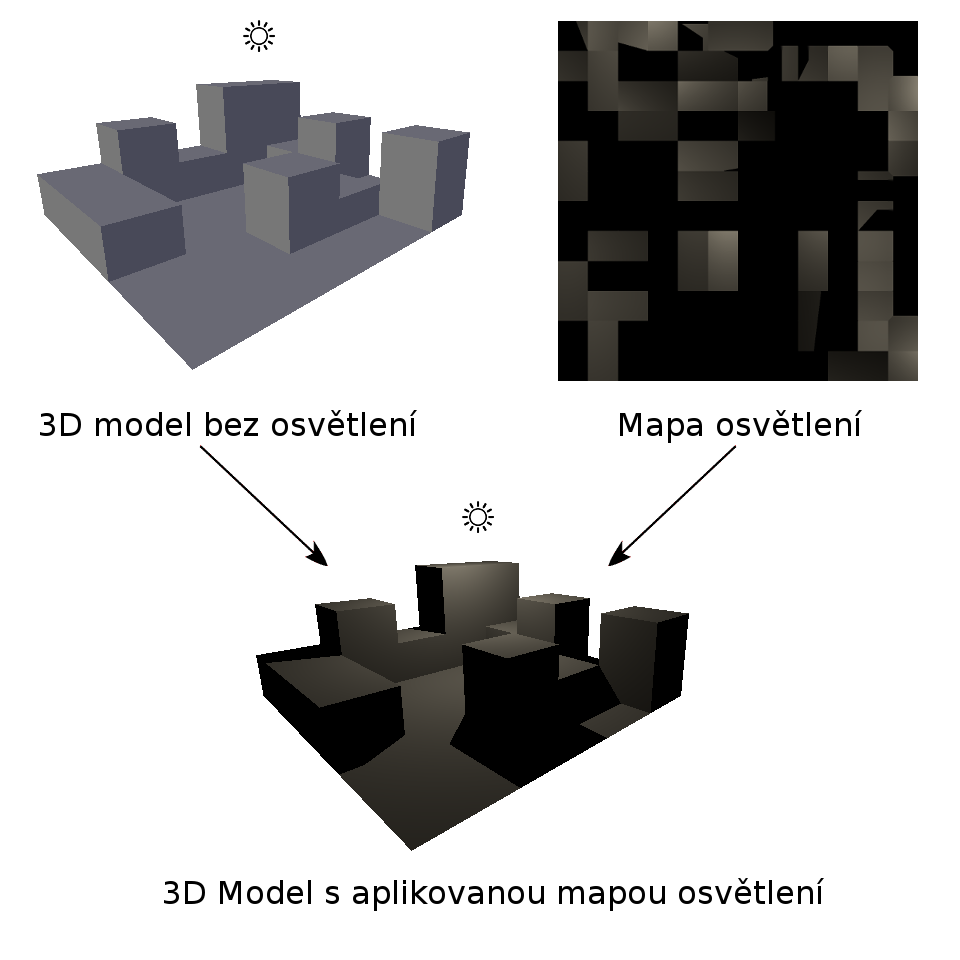
\includegraphics[width=100mm]{figures/lmapply.png}
\caption{Ukázka mapy osvětlení na jednoduchém 3D modelu}
\end{figure}
\end{center}

Aby bylo možné mapy osvětlení dynamicky aktualizovat, je potřeba mít do map rychlý zapisovací přístup. Rychlé zapisování do textur se v OpenGL realizuje pomocí Frame Buffer Objektu (FBO). Pro aktualizaci musíme mít předpočítanou tzv. záplatu. Záplatou se rozumí menší textura, která se přidá do současné osvětlovací mapy. Přidáním záplaty lze tedy přidat do scény další světlo, které máme předpočítané. Záplata jde z FBO opět odebrat (provede se odečet stejné záplaty).

Protože uchovávání záplat v paměti by bylo příliš paměťově náročné, jsou uloženy\linebreak ve vektorové podobě přímo na GPU pomocí Vertex Buffer Objektu (VBO). 
\newpage

\begin{center}
\begin{figure}[h!]
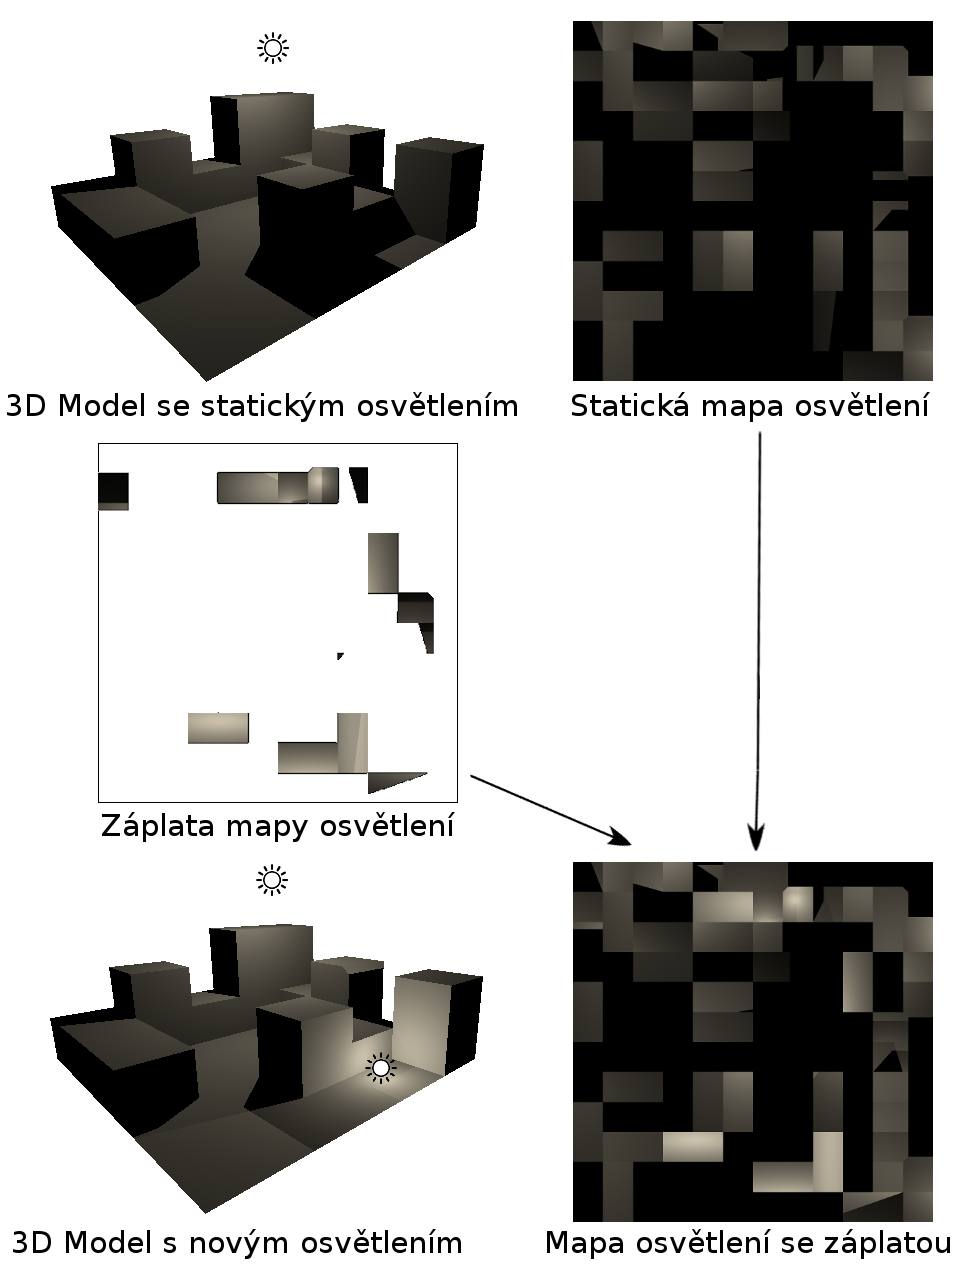
\includegraphics[width=110mm]{figures/lmupdate.png}
\caption{Ukázka aktualizace map osvětlení na jednoduchém 3D modelu}
\end{figure}
\end{center}

\subsection{Statické osvětlení s dynamickými objekty ve scéně}
Při použití dynamických objektů ve scéně se statickém osvětlením vznikají dva základní problémy. Prvním problém je, že dynamické objekty mají jiné osvětlení než statická scéna\linebreak a to vypadá velice nepřirozeně. Druhým problémem je, že pokud dynamický objekt zastíní zdroj světla, tak nevznikne stín na statických objektech.

Oba problémy lze vyřešit jen částečně. V prvním případě lze přečíst informaci o intenzitě osvětlení z nejbližšího bodu na statickém objektu a tuto intenzitu aplikovat na dynamický objekt. V druhém případě při vykreslování jednotlivých pixelů lze zjistit, zda se v okolí vykreslovaného bodu nenachází dynamický objekt a tím aproximačně zjistit, zda byl vykreslovaný bod zastíněn.
\newpage

\section{Cílová platforma Android}
Platforma Android je postavena na Linuxovém jádře a využívá knihovny, které bývají součástí unixových systémů. Od klasického desktopového Linuxu se odlišuje hlavně v tom, že jako hlavní programovací jazyk využívá Javu. Pomocí Javy je naprogramováno celé Android API, které zprostředkovává téměř veškeré služby systému.

Na Androidu je téměř nemožné spustit C/C++ program přímo. Standardně se to řeší tak, že se vytvoří z programu knihovna, kterou spustí kód napsaný v Javě. Pak je nutné veškeré vstupy/výstupy obsluhovat v jazyce Java a to velice komplikuje portování programů z desktopového Linuxu na Android. Výjimku tvoří OpenGL, které umožňuje vykreslovat\linebreak na displej přímo z C/C++ kódu.

\begin{center}
\begin{figure}[h!]
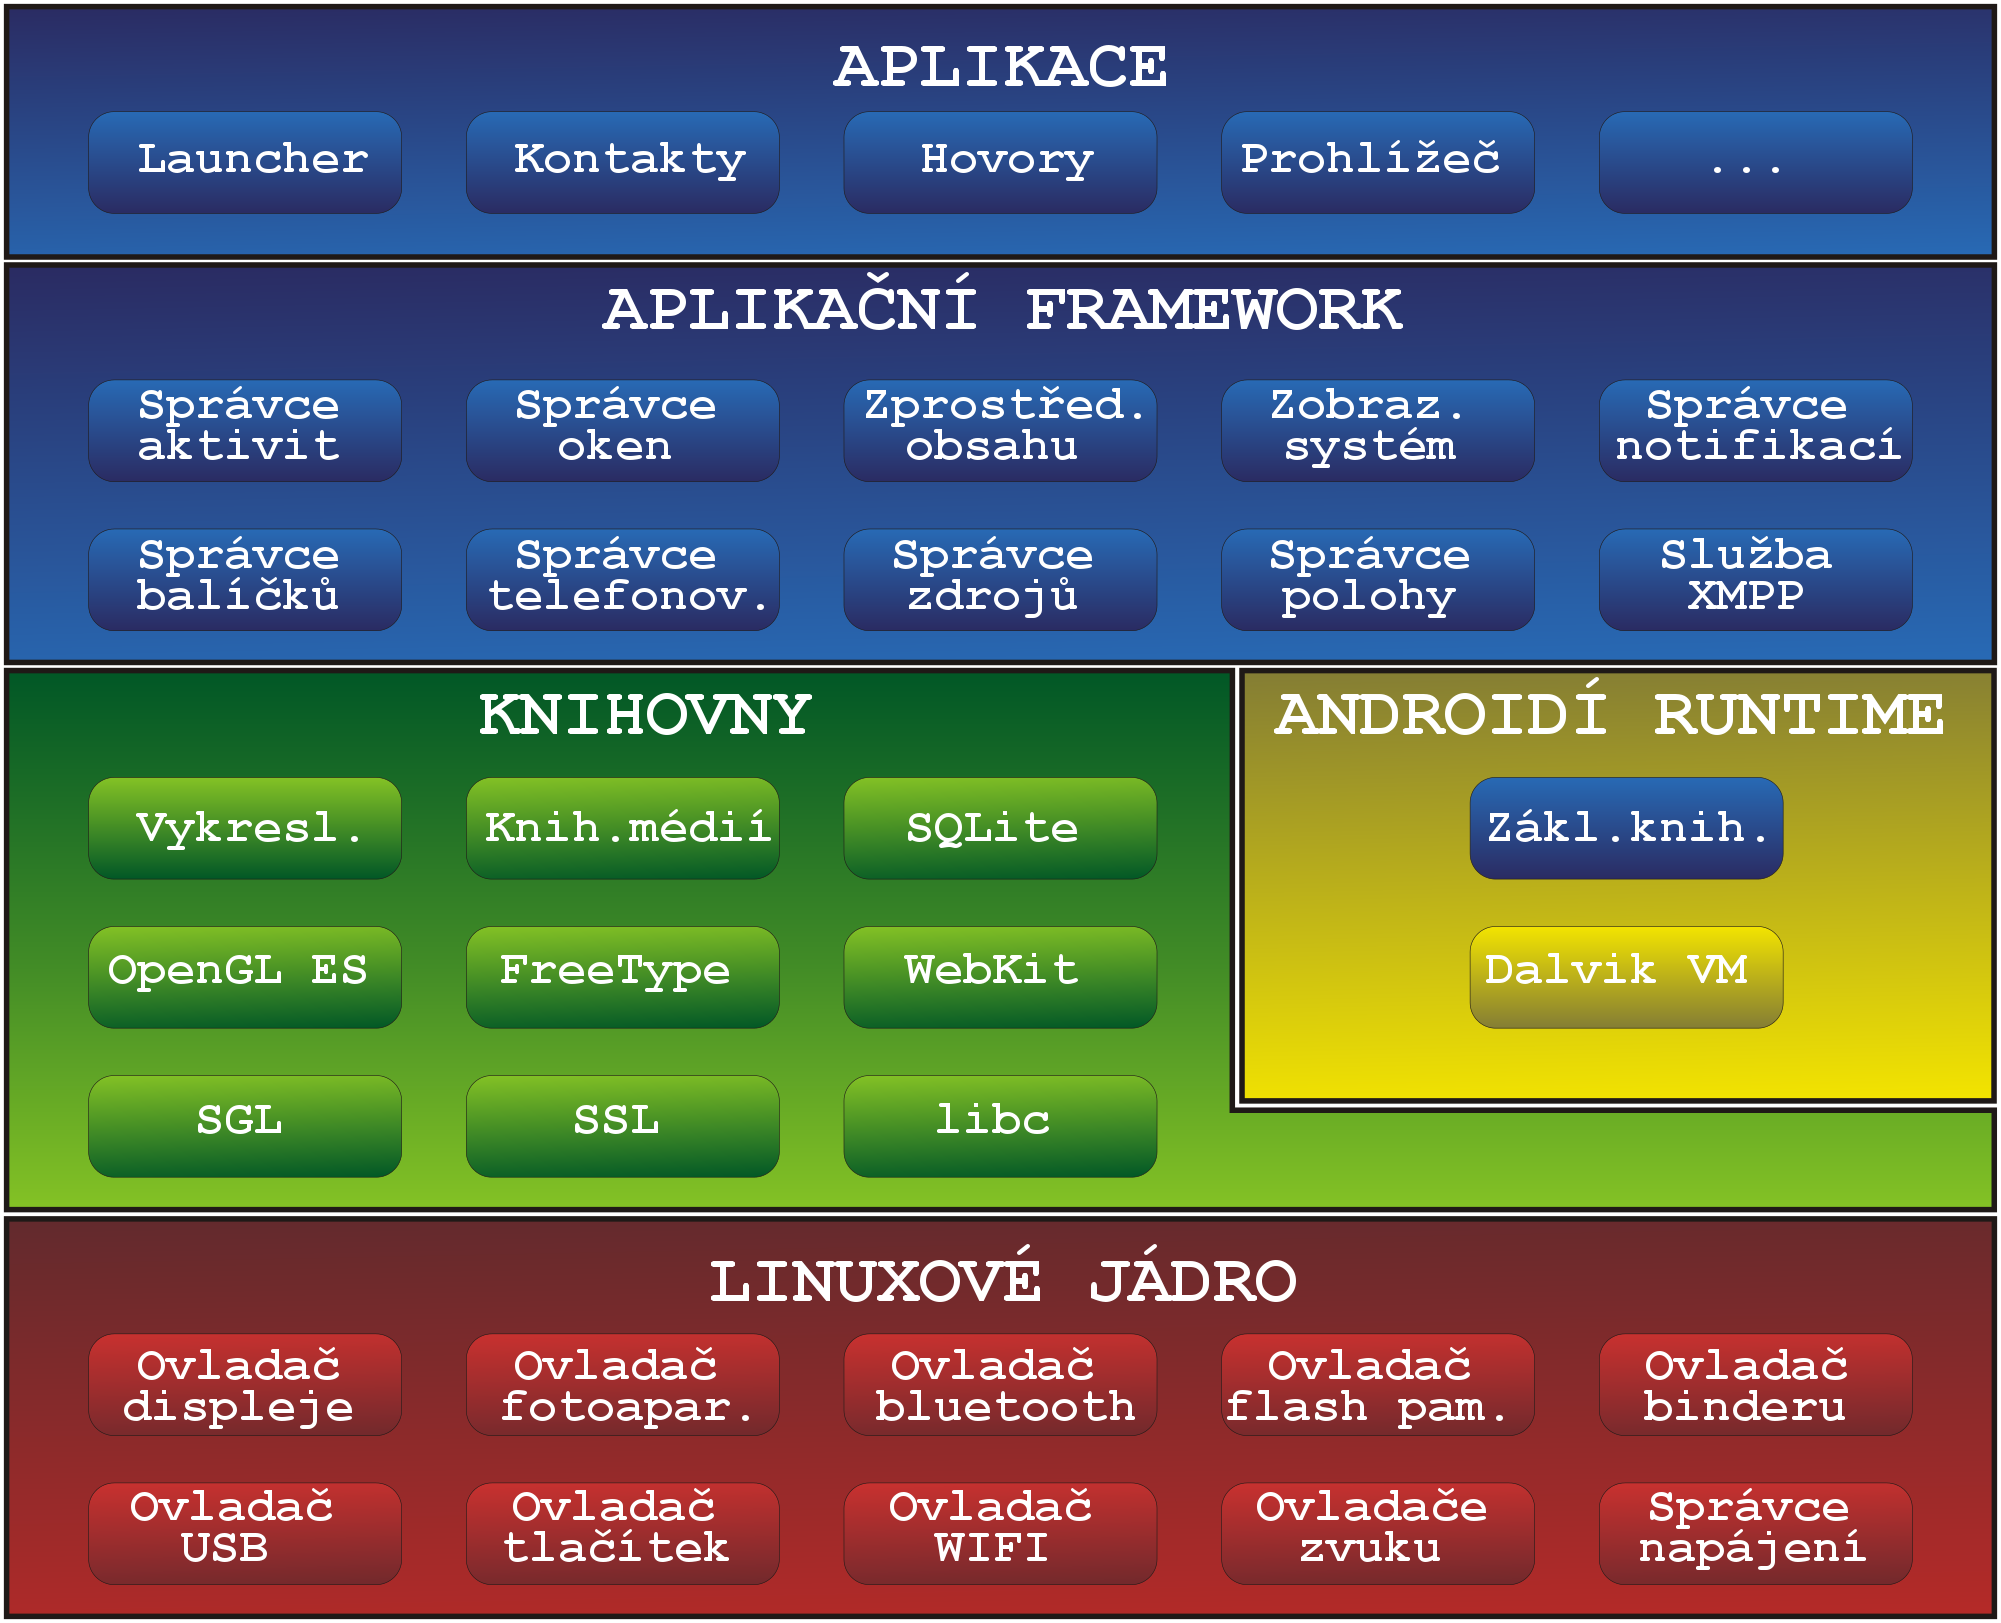
\includegraphics[width=120mm]{figures/android.png}
\caption{Komponenty platformy Android, komponenty vyznačené modrou barvou jsou napsané v jazyce Java, žlutou barvou je virtuální stroj, který umožňuje běh Java aplikací, zelenou barvou jsou C/C++ knihovny a červenou je Linuxové jádro}
\end{figure}
\end{center}

Pro platformu Android existuje nepřeberné množství aplikací a toho začínají využívat ostatní platformy. V současné době platformy BlackBerry a Jolla umožňují spouštět Android aplikace, dále existuje platforma NokiaX, která je postavena přímo na operačním systému Android.

\section{Existující implementace}

Rešerši existujících implementací jsem zaměřil na dvě různé kategorie. První kategorie jsou implementace pro PC, kde je nejčastěji řešeno nepřímé osvětlení, které by na mobilních zařízeních zatím použít nešlo. Druhá kategorie jsou závodní simulátory s noční jízdou pro platformu Android. V této kategorii bývají nejčastěji použity techniky jako v této práci.

\subsection{Projekty zabývající se vykreslování noční scény}

V této sekci jsem vybral co nejrealističtější implementace, ke kterým existuje nějaký článek o tom, jak bylo výsledku dosaženo. Existuje sice několik implementací, které vypadají ještě více realističtěji. To jsou ale většinou komerční produkty, které nesdílejí ostatním, jakým způsobem byla implementace realizována.

\subsubsection{Proceduralní modelování města a osvětlení nočního města}
Tato implementace je z roku 1999 a zabývá se proceduálním modelováním města (konkrétně Bostonu) a následně jej vykresluje pomocí sledování paprsku za využití algoritmu Monte Carlo. Implementace pochopitelně neběží v reálném čase. Výsledek je při detailním záběru po grafické stránce velice realistický. Vytknul bych jen, že reflektory vozidla osvítí pouze blízké okolí. Při záběru na město z výšky výsledek nebudí tolik realistický dojem jako při detailním záběru.

\begin{center}
\begin{figure}[h!]
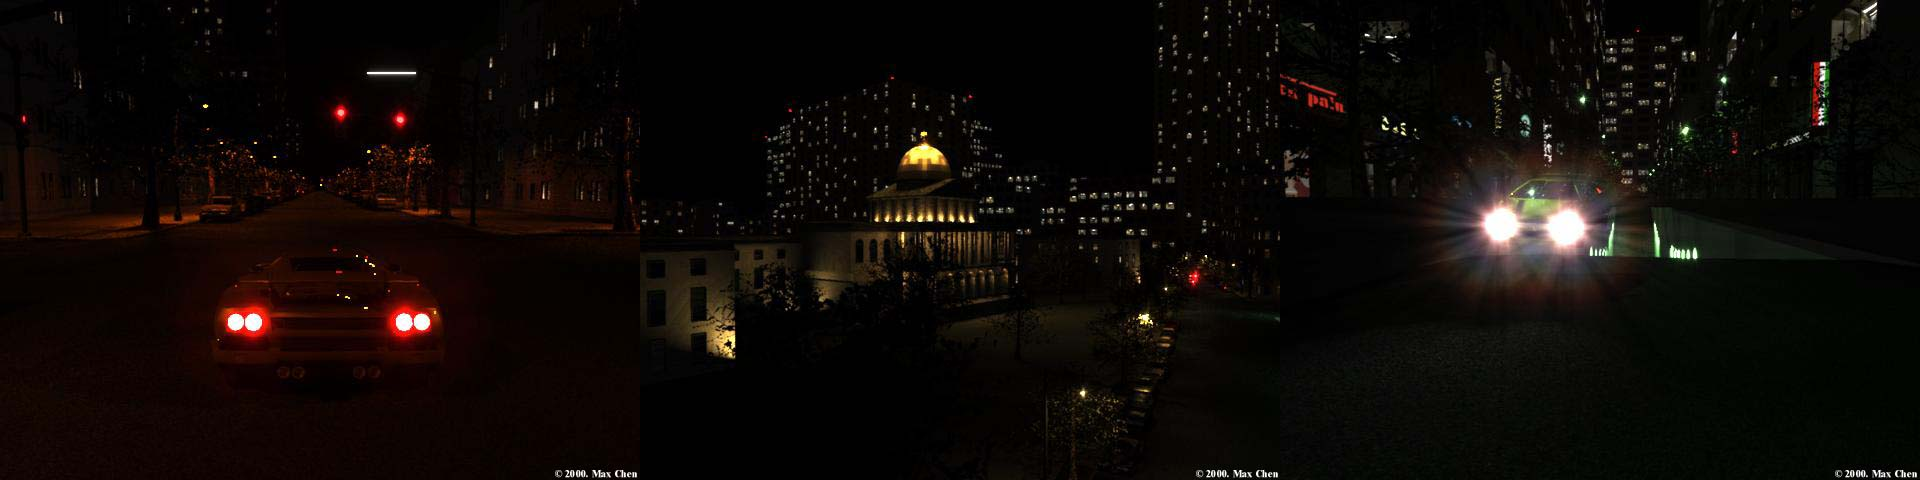
\includegraphics[width=150mm]{figures/NR.png}
\caption{Ukázka nočního renderingu}
\end{figure}
\end{center}
\newpage

\subsubsection{Imperfektní stínové mapy pro výpočet nepřímého osvětlení}
Tato implementace, představená roku 2008, se nezabývá přímo noční scénou, zabývá se nepřímým osvětlením, které s noční scénou souvisí. Implementace běží v reálném čase a její výsledky jsou srovnatelné se snímky, které se vykreslují několik hodin.

V této implementaci se nevyužívá předpočtených dat. Využívá se zde virtuálních bodových světel (VPL), která simulují odrazy světla. Z každého VPL se vytvoří stínová mapa o malém rozlišení a při vykreslování výsledné scény se vyhodnocuje viditelnost ze všech VPL.

Implementace podporuje více typů zdrojů světla, včetně plošných. Nemá problémy\linebreak s barevným světlem ani s kaustiky.

\begin{center}
\begin{figure}[h!]
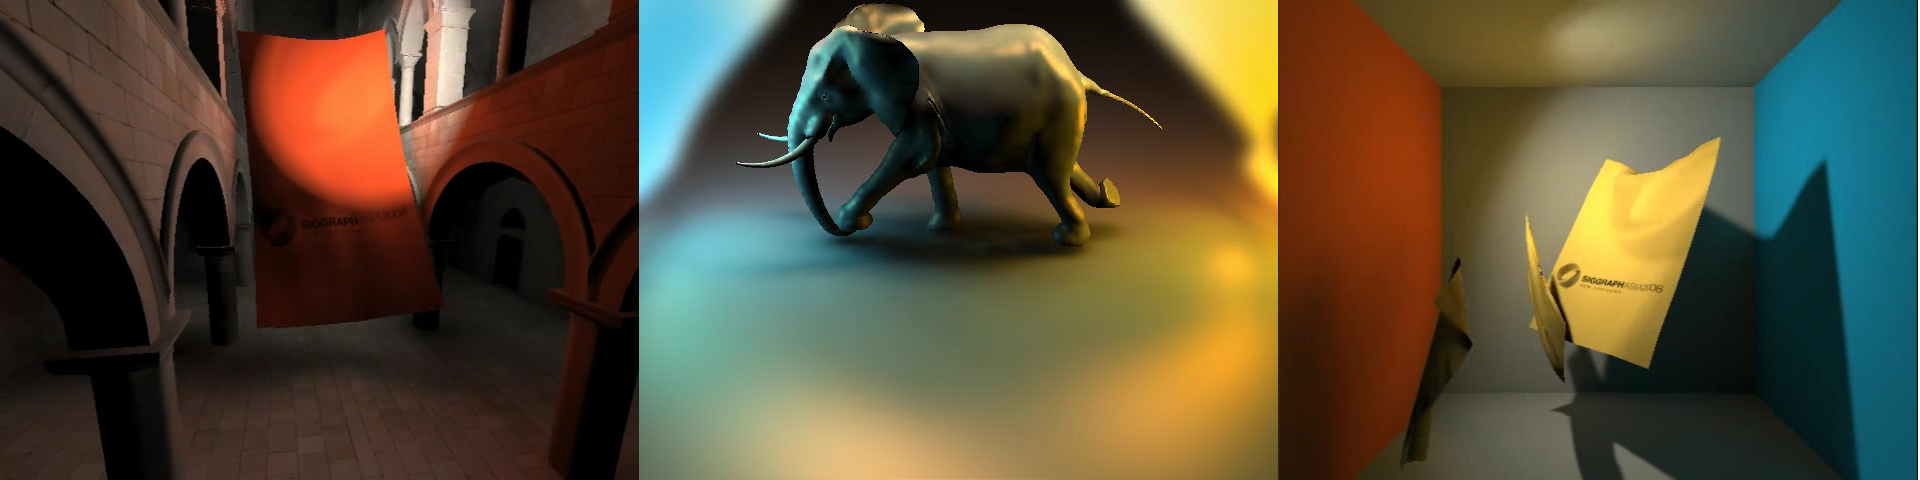
\includegraphics[width=150mm]{figures/ISM.png}
\caption{Ukázka výsledků techniky imperfektních stínových map pro efektivní výpočet nepřímého osvětlení}
\end{figure}
\end{center}

\subsection{Závodní simulátory s noční scénou pro platformu Android}
V této sekci jsem vyhledával i implementace, u kterých není uvedeno, jak bylo výsledků dosaženo. Je to z důvodu malého počtu implementací odpovídající dané kategorii.

\subsubsection{Asphalt Urban od Gameloftu}
Asphalt Urban je série mobilních závodních simulátorů, jejíchž první díl byl publikován spolu s herním smartphonem Nokia N-Gage. Jedná se o úspěšnou sérii, která přitahuje hráče všech možných platforem.

Zmíním 7.díl ze série Asphalt Urban, který osobně považuji za nejúspěšnější díl. Osvětlení z pouličních lamp je součástí textur, reflektor vozidla je tvořen zřejmě pomocí projektivní textury. Povrch zrcadlově odráží 3D objekty. Po bližším zkoumání lze zjistit, že některé tyto odražené objekty jsou odlišné. Domnívám se, že zde byl použit duplicitní objekt.

Další díl ze série Asphalt Urban už odlesky řeší lépe. Odráží se hlavně světla a odlesk je lépe přizpůsoben povrchu. Vzniká zde dojem mokré silnice. Dochází i k rozmazání brzdových světel. Osvětlení od lamp je opět řešeno texturou. Nepříjemnou změnou je absence reflektoru vozidla a přidání rušivého chvění kamery během jízdy.

\subsubsection{Need for Speed Most Wanted od EA Games a Firemonkeys}
Simulátor, který je spíše známý z PC, na mobilním trhu takový úspěch nemá. Od PC verze je velice odlišný, ale rozhodně se nejedná o nějakou lacinou napodobeninu. Jedná se o první závodní simulátor pro mobilní zařízení, který disponuje modelem ničení vozidla (je možné vozidlo poškrábat, rozbít mu okna apod).

Oproti Asphalt 8 má navíc efekt Depth-of-field. To znamená, že vzdálené modely jsou rozmazané a zabarveny do barvy pozadí. Tento efekt vytváří příjemný mlhovitý dojem. Jinak bych řekl, že tyto dva simulátory jsou si sobě velice podobné. Na stejném enginu funguje\linebreak i známý simulátor Real Racing 3, který ale noční jízdu nemá.

\subsubsection{GT Racing 2 od Gameloftu}
Úspěšným závodním simulátorem je v současné době GT Racing 2, je to hlavně díky jeho zpracování. Jako jediný z uvedených simulátorů má při noční jízdě nízké ambientní osvětlení a scéna je osvětlena hlavně reflektorem vozidla.

Nejsem si jist, zda osvětlení lampami je přímo součástí textur nebo jestli jsou zde použity mapy osvětlení.

\subsubsection{Sports Car Challenge od Fishlabs}
Asi nejdetailnější model vozidla má právě Sports Car Challenge. Vývojář spolupracuje s předními výrobci automobilů a to se odrazilo právě na modelech vozidel. Modely jsou realistické a to včetně interiérů.

Projekt trpí slabší kompatibilitou s mobilními zařízeními, i když náročnost enginu je nízká. Co se týká noční jízdy, je realizována stejnými technikami jako denní jízda. Jsou zde použity pouze tmavé textury a halo efekt pouličních lamp.

\subsubsection{Track Racing od vývojáře Soulkey}
I když tento projekt není závodní simulátor s noční jízdou, zmiňuji ho hlavně kvůli ovládání. Jedná se o neoficiální remake hry Trackmania známé z PC. Projekt běží na Unity3D enginu a je dostupný na mnoha platformách, nedá se ale stáhnout přímo z Marketu či Storu.

U výše uvedených simulátorů vozidlo automaticky zrychluje a u některých i samo brzdí. Hráč nemá tedy nad vozidlem takovou kontrolu. V případě Track Racing má hráč nad vozidlem plnou kontrolu a zážitek ze hry se dá srovnat se zážitkem z původní PC hry.
\newpage

\begin{center}
\begin{figure}[h!]
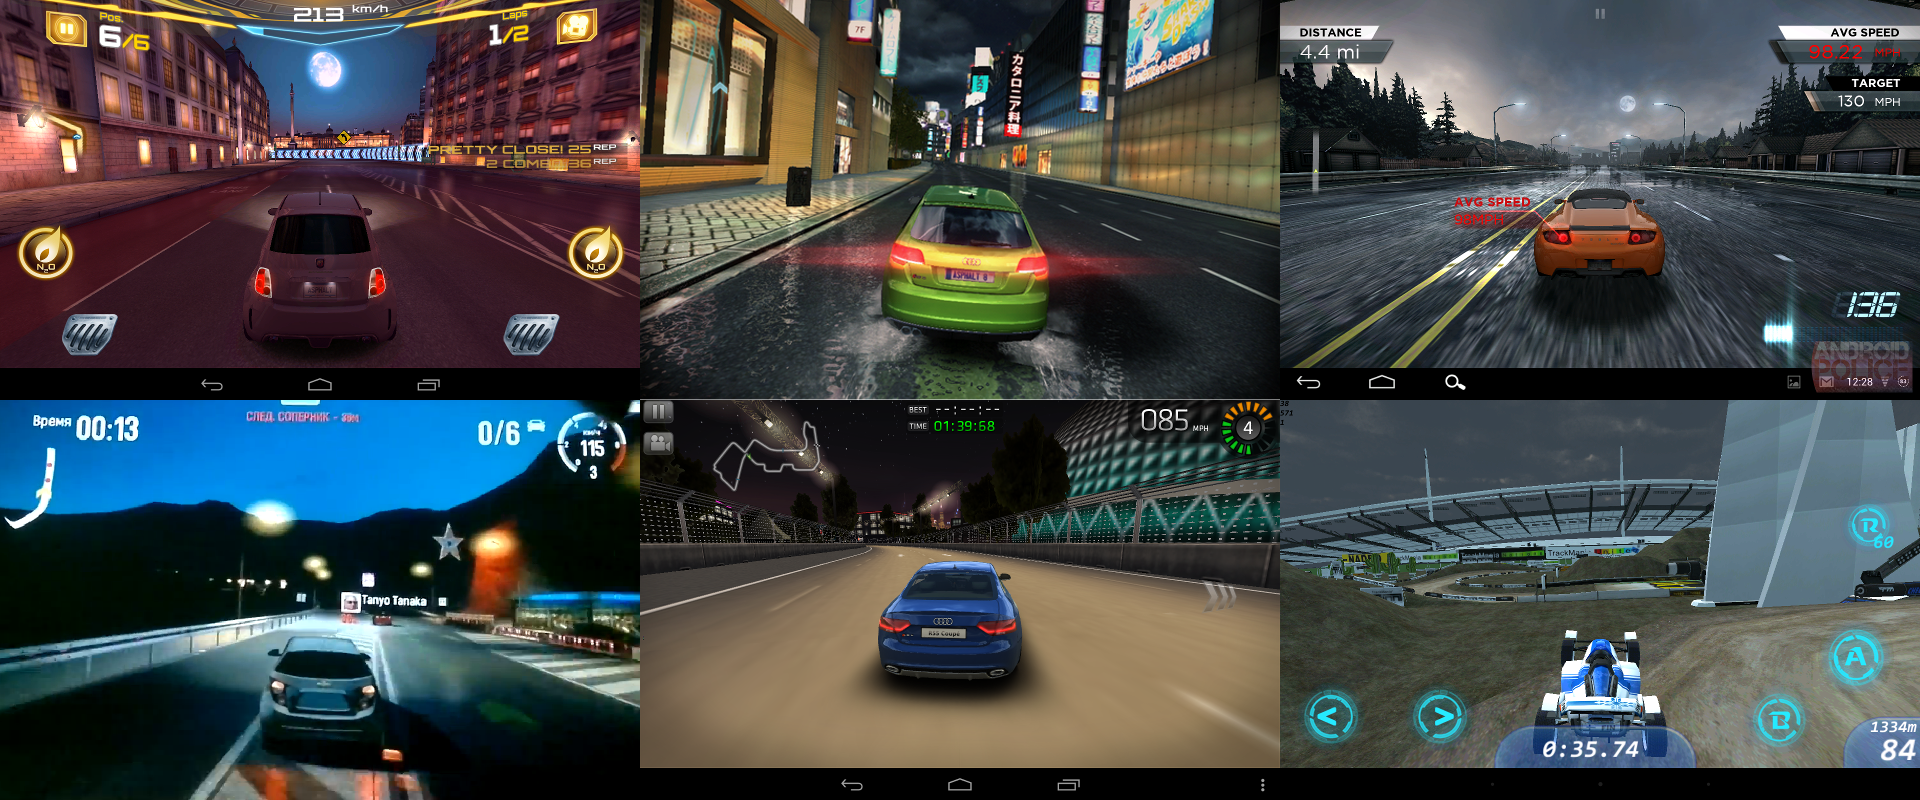
\includegraphics[width=150mm]{figures/games.png}
\caption{Ukázka závodních simulátorů s noční scénou pro platformu Android, první řada zleva: Asphalt 7, Asphalt 8, Need for Speed Most Wanted, druhá řáda zleva: GT Racing 2, Sports Car Challenge, Track Racing}
\end{figure}
\end{center}

%*****************************************************************************
\chapter{Teoretická část}

\section{Osvětlovací model}
Existuje několik osvětlovacích modelů, asi nejpoužívanější lokální osvětlovací model je Phongův. Phongův model se skládá ze tří typů osvětlení.
\begin{itemize}
\item ambientní osvětlení - nahrazuje nepřímé osvětlení konstantní hodnotou osvětlení
\item difúzní osvětlení - osvětlení nezávislé na pohledu kamery, Odpovídá ideálně matnému povrchu
\item spekulární osvětlení - osvětlení závislé na pohledu kamery, odpovídá ideálně odrazivému povrchu
\end{itemize}

Jak je patrné z obrázku 3.1, výsledná intenzita osvětlení povrchu $I$ je součtem ambientní složky ($I_a$), difúzní složky ($I_d$) a spekulární složky ($I_s$).
\begin{center}
$I = I_a + I_d + I_s$
\end{center}

\begin{center}
\begin{figure}[h!]
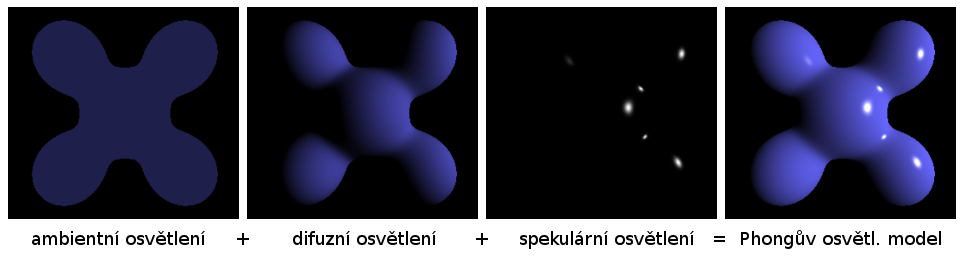
\includegraphics[width=150mm]{figures/phong.png}
\caption{Phongův osvětlovací model}
\end{figure}
\end{center}

Všesměrové osvětlení je ve Phongovo osvětlovacím modelu konstantní pro daný objekt\linebreak a říká se jí ambientní osvětlení $I_a$. Výsledná intenzita se spočte jako součin barvy ambientního světla $C_a$, koeficientem ambientního odrazu $k_a$ a barvou povrchu $C_d$, která je shodná i pro difúzní složku.
\begin{center}
$I_a = C_a \cdot k_a \cdot C_d$
\end{center}

Difúzní složka odpovídá ideálně matnému (Lambertovskému) povrchu a závisí na úhlu $\alpha$ mezi vektory $\vec{L}$ a $\vec{N}$.
\begin{center}
\begin{figure}[h!]
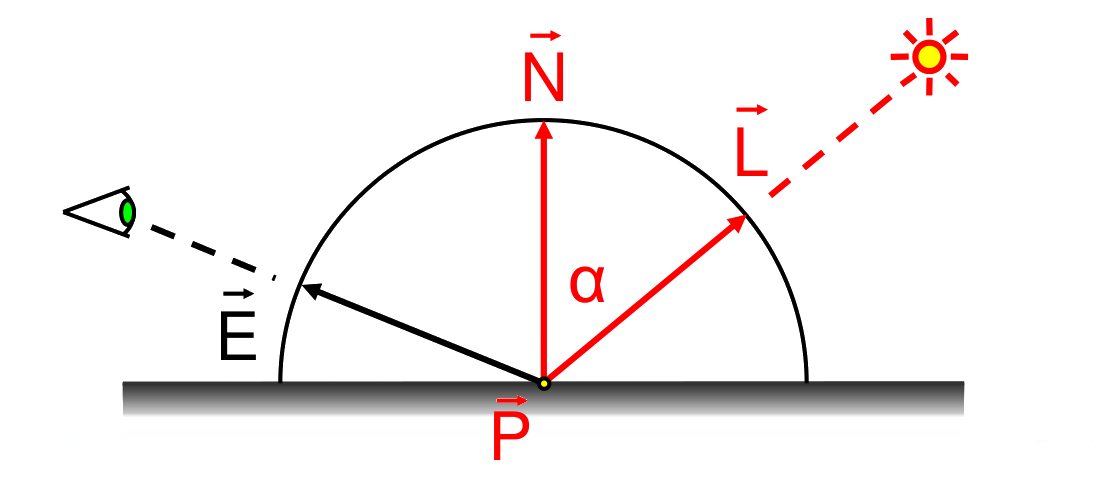
\includegraphics[width=60mm]{figures/phongD.png}
\caption{Vektory k výpočtu difúzního osvětlení, $\vec{L}$ je normalizovaný směr světla, $\vec{N}$ je normalizovaná normála povrchu, $\alpha$ je úhel, který tyto vektory svírají, $\vec{E}$ je normalizovaný směr pohledu kamery (eye vektor) a $\vec{P}$ je bod na povrchu tělesa}
\end{figure}
\end{center}
Intenzitu difúzní složky lze vyjádřit následovně.
\begin{center}
$I_d = C_l \cdot k_d \cdot C_d \cdot cos(\alpha)$
\end{center}
$C_l$ je barva světla, $k_d$ koeficient difúzního odrazu, $C_d$ barva povrchu a pro úhel $\alpha$ platí, že $cos(\alpha) = \vec{L} \cdot \vec{N}$. Po dosazení tedy získáme výsledný výraz.
\begin{center}
$I_d = C_l \cdot k_d \cdot C_d \cdot (\vec{L} \cdot \vec{N})$
\end{center}
\bigskip

Spekulární (zrcadlová) složka odpovídá ideálně odrazivému tělesu a závisí na úhlu $\beta$ mezi vektory $\vec{E}$ a $\vec{R}$. 
\begin{center}
\begin{figure}[h!]
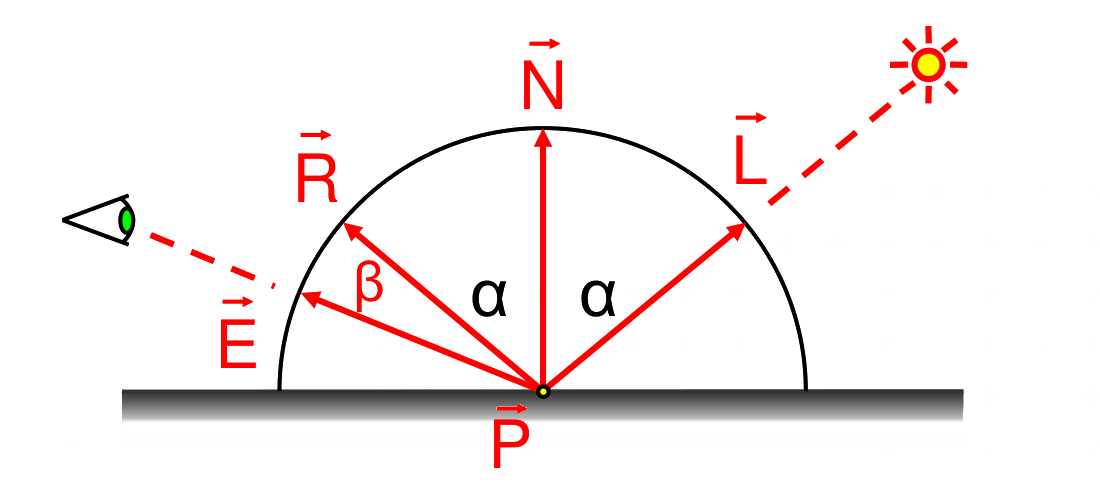
\includegraphics[width=60mm]{figures/phongS.png}
\caption{Vektory k výpočtu spekulárního osvětlení, $\vec{E}$ je normalizovaný směr pohledu kamery (eye vektor), $\vec{R}$ je normalizovaný směr odrazu světla, $\beta$ je ůhel, který tyto vektory svírají a $\vec{P}$ je bod na povrchu tělesa}
\end{figure}
\end{center}
Intenzitu spekulární složky lze vyjádřit následovně.
\begin{center}
$I_s = C_l \cdot k_s \cdot C_s \cdot cos^h(\beta)$
\end{center}
$C_l$ je barva světla, $k_s$ koeficient spekulárního odrazu, $C_s$ barva lesklého povrchu (většinou bývá bílá), $h$ je ostrost odrazu a pro úhel $\beta$ platí, že $cos(\beta) = \vec{E} \cdot \vec{R}$. Po dosazení tedy získáme výsledný výraz.
\begin{center}
$I_s = C_l \cdot k_s \cdot C_s \cdot (\vec{E} \cdot \vec{R})^h$
\end{center}

\section{Výpočet osvětlení}

Pro výpočet osvětlení konkrétního bodu na obrazovce je potřeba nejdříve spočítat příspěvky jednotlivých světel pro tento bod. Příspěvky jednotlivých světel spočteme jako součin efektivity reflektoru pro daný vertex $E_r$, faktoru útlumu $F_a$ a součtu složek Phongova osvětlovacího modelu.
\begin{center}
$light_i = E_r \cdot F_a \cdot (I_a + I_d + I_s)$
\end{center}

Efektivita reflektoru $E_r$ je parametr určující intenzitu osvětlení zdroje světla typu reflektor. Příkladem takového zdroje světla je například baterka.
\begin{center}
\begin{figure}[h!]
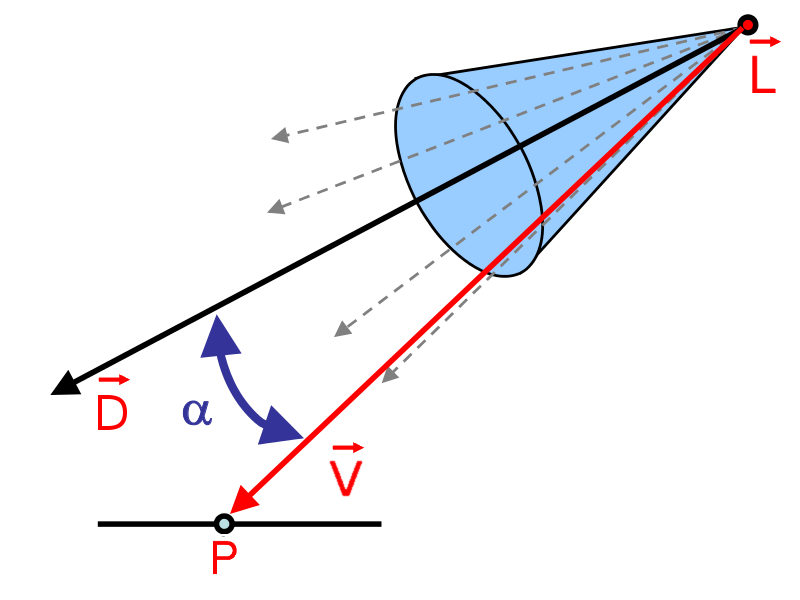
\includegraphics[width=60mm]{figures/cutoff.png}
\caption{Vektory k výpočtu efektivity reflektoru, $\vec{D}$ je normalizovaný směr světla, $\vec{V}$ je normalizovaný směr světla na kraji světelného kužele, $\alpha$ je úhel, který tyto vektory svírají, $\vec{L_p}$ je pozice zdroje světla a $\vec{P}$ je bod na povrchu tělesa}
\end{figure}
\end{center}

Hodnota efektivity reflektoru se spočte podle následujících podmínek.\\
Pokud světlo není reflektor, poté $E_r = 1$.\\
Pokud bod leží mimo světelný kužel, tedy $(\vec{V} \cdot \vec{D}) < cos(\alpha)$, poté $E_r = 0$.\\
Pro ostatní případy $E_r = max(0, cos(\vec{V} \cdot \vec{D}))^{k_{se}}$, kde $k_{se}$ je parametr spot efektu.
\newpage

Faktor útlumu $F_a$ řeší, jak moc má být intenzita světla utlumena s rostoucí vzdáleností $d$ od zdroje světla. Konstantní útlum určuje parametr $k_c$, lineární útlum parametr $k_l$\linebreak a kvadratický útlum parametr $k_q$.
\begin{center}
$F_a = \frac{1}{k_c + k_l \cdot d + k_q \cdot d^2}$
\end{center}
\bigskip

Výsledná barva bodu na obrazovce se spočítá jako součet barvy emisního světla $C_e$, barvy globálního ambientního světla $C_{ag}$ a sumy příspěvků jednotlivých světel.
\begin{center}
$color = C_e + C_{ag} + \sum_{}{} light_i$
\end{center}

\section{Stínování}
Pojem stínování v počítačové grafice znamená postup vybarvování trojúhelníků. Existují tři typy stínování.
\begin{itemize}
\item Konstantní stínování - celý polygon se vybarví jednou barvou dle normály povrchu. Používá se ve scénách, ve kterých se nacházejí pouze směrové zdroje světla.
\item Gouraudovo stínování - spočítá se osvětlení ve vrcholech a následně se interpolují hodnoty mezi vrcholy. Toto stínování je velmi rychlé. Problém nastane, pokud světlo osvětluje střed polygonu a zároveň neosvětluje nebo jen částečně osvětluje vrchol. Osvětlení je po té ve vrcholech velmi nízké a nemůže tedy vzniknout korektně osvětlený obraz.
\item Phongovo stínování - spočítá se osvětlení pro každý pixel polygonu na obrazovce. Dnes je to asi nejpoužívanější stínování. V OpenGL se toto stínování provádí pomocí shaderů. Vstupem do vertexového shaderu je pozice vrcholu a jeho normála. Ve vertex shaderu se provede transformace do pohledu kamery a určí se, že pozice vrcholu a normála se mají interpolovat. Po rasterizaci získáme interpolované hodnoty jako vstup ve fragment shaderu a zde provedeme výpočet podle výše uvedeného osvětlovacího modelu.
\end{itemize}

\begin{center}
\begin{figure}[h]
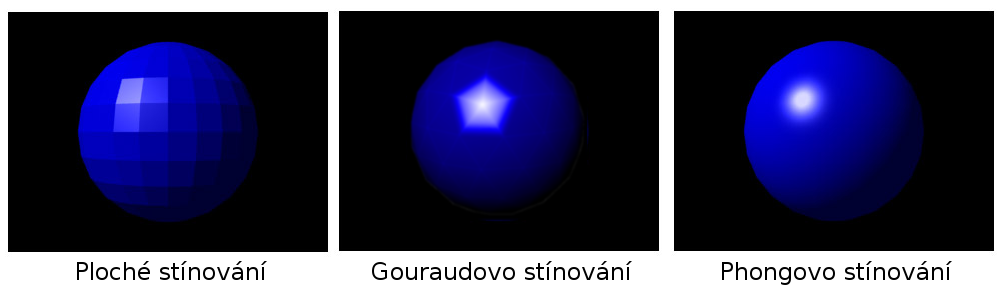
\includegraphics[width=135mm]{figures/shading.png}
\caption{Ukázka jednotlivých typů stínování}
\end{figure}
\end{center}
\newpage

Interpolaci provádí OpenGL automaticky. Jeden ze způsobů jak provést interpolaci ručně je provést rasterizaci(tím získat všechny body uvnitř trojúhelníka) a poté provést barycentrickou interpolaci.

\begin{center}
\begin{figure}[h]
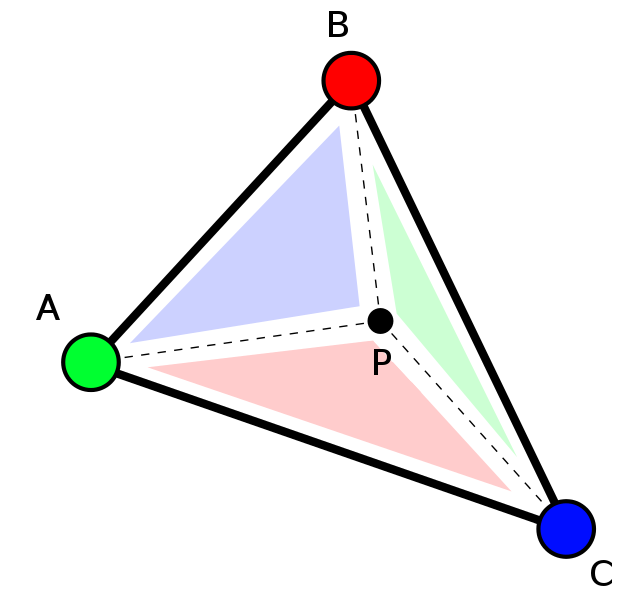
\includegraphics[width=65mm]{figures/interpolation.png}
\caption{Pomocný obrázek k výpočtu barycentrické interpolace}
\end{figure}
\end{center}

Nejdříve potřebujeme spočítat obsah jednotlivých trojúhelníků, abychom získali váhu hodnot v jednotlivých vrcholech.
\begin{center} 
$S_{PBC} = \frac{|\vec{PB} \times \vec{PC}|}{2}$;
$S_{APC} = \frac{|\vec{AP} \times \vec{AC}|}{2}$; 
$S_{ABP} = \frac{|\vec{AB} \times \vec{AP}|}{2}$;
$S_{ABC} = \frac{|\vec{AB} \times \vec{AC}|}{2}$
\end{center}

Pokud si označím hodnotu u bodu $A$ jako $a$, u bodu $B$ jako $b$ a u bodu $C$ jako $c$, získáme interpolovanou hodnotu $p$ v bodě $P$ následovně.
\begin{center}
$p = a \cdot \frac{S_{PBC}}{S_{ABC}} + b \cdot \frac{S_{APC}}{S_{ABC}} + c \cdot \frac{S_{ABP}}{S_{ABC}}$
\end{center}

\section{Míchání textur}

Míchání textur se v OpenGL provádí pomocí blendingu. Tato technika míchá cílový obraz (ten již vykreslený ve FBO) a zdrojový obraz, tedy texturu namapovanou na nějaký model.

Vstupem pro blending funkci je zdrojová barva $C_s$, cílová barva $C_d$ a parametry $B_s$\linebreak a $B_d$, které určují pro každý kanál, jak se má hodnota míchat. Výstupem funkce je nová cílová barva $C_d$.
\begin{center}
$C_d = C_s \cdot B_s + C_d \cdot B_d$
\end{center}

Příklad použití blendingu je technika poloprůhledného materiálu. Nejdříve se vykreslí neprůhledná část scény (tím se vykreslí i hloubkový buffer). Poté se vypne zápis do hloubkového bufferu a vykreslí se geometrie s částečnou průhledností.

\begin{figure}[h]
\begin{center}$
\begin{array}{cc}
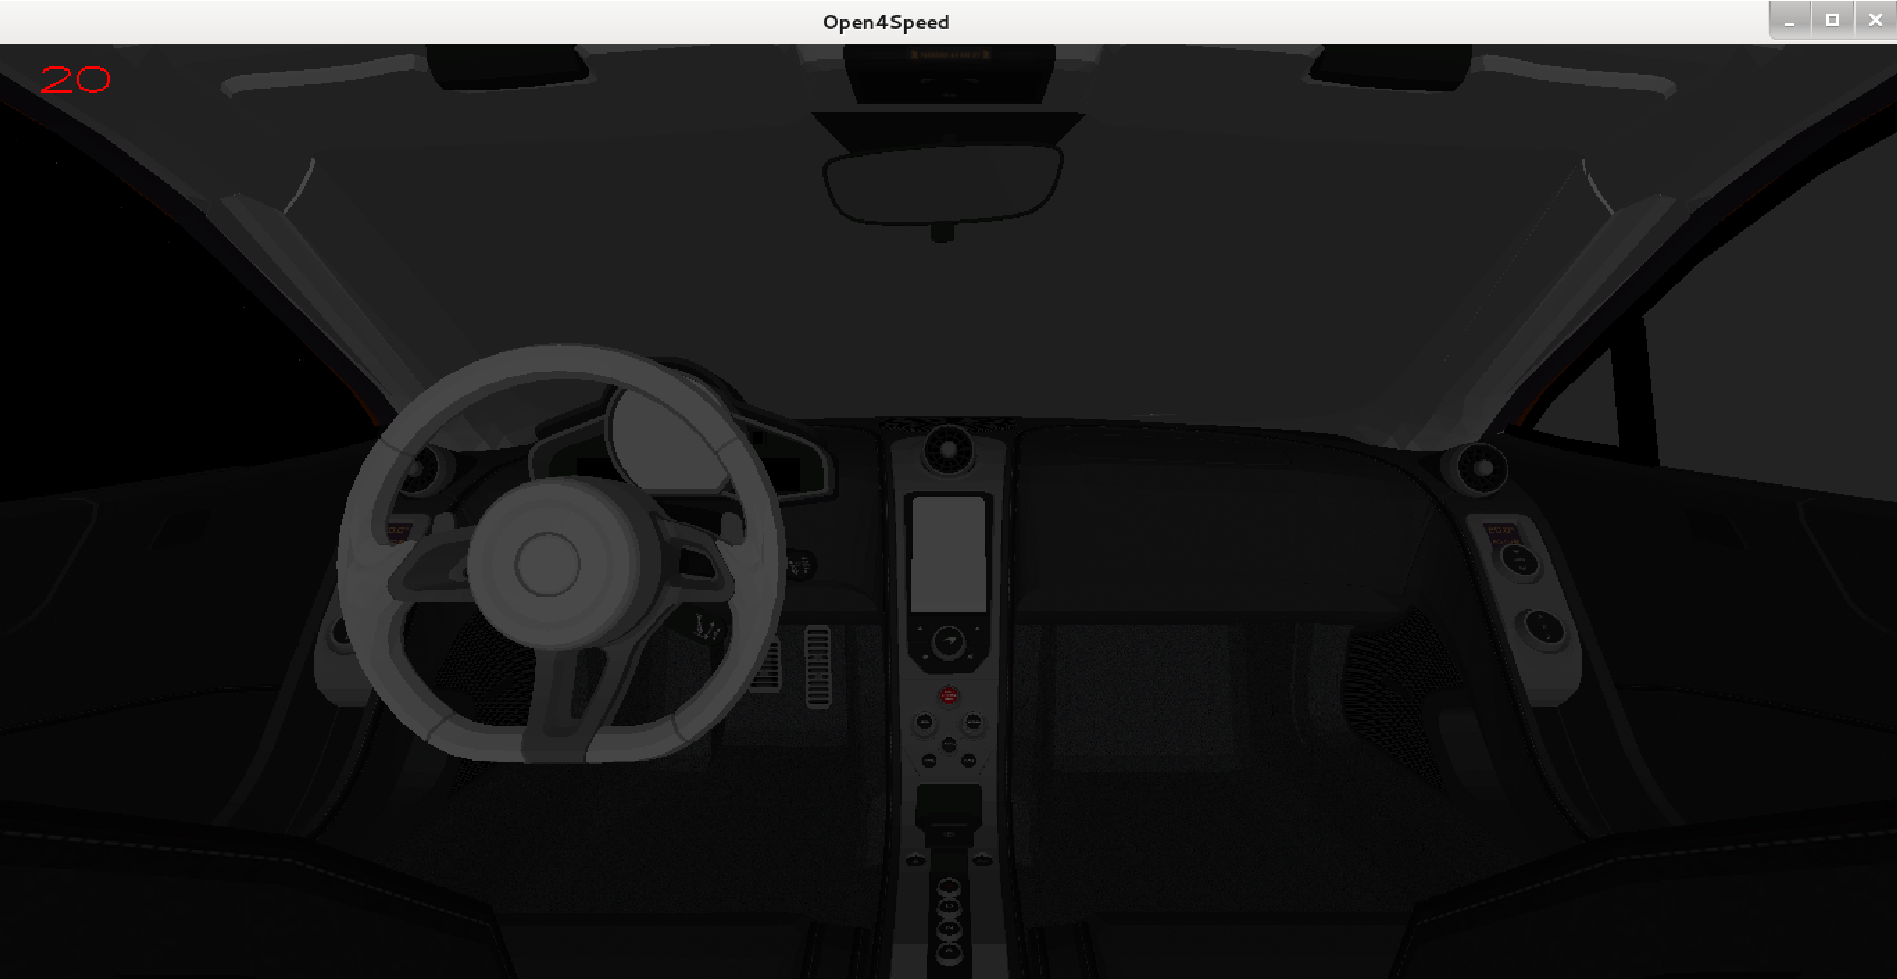
\includegraphics[width=60mm]{figures/blendoff.png} &
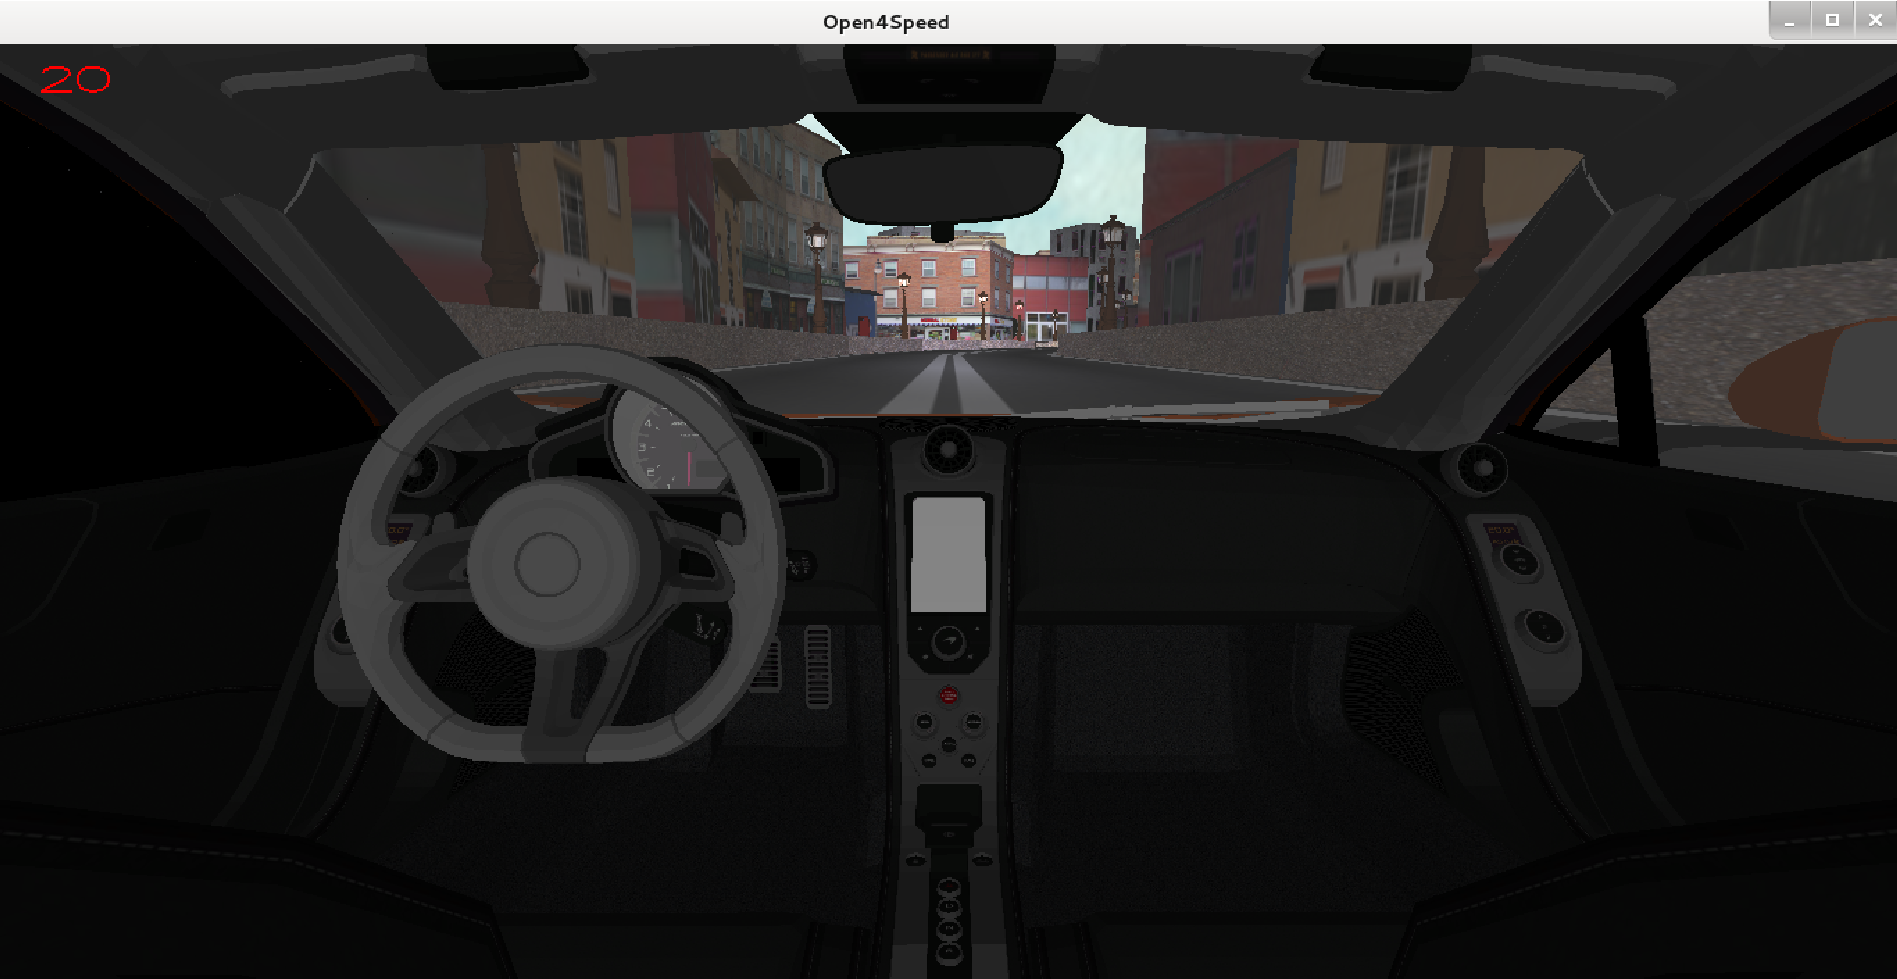
\includegraphics[width=60mm]{figures/blendon.png}
\end{array}$
\end{center}
\caption{Ukázka problému při vykreslení poloprůhledného materiálu před neprůhledným}
\end{figure}

\section{Výpočet stínů v reálném čase}
Stíny v počítačové grafice napomáhají k vnímání souvislostí ve scéně. Pokud ve scéně stíny nepoužijeme, nebudeme například schopni poznat, zda se těleso dotýká povrchu nebo se vznáší (výjimku tvoří pohled, při kterém vzniká viditelná mezera mezi objektem a povrchem).

Abychom mohli stín spočítat, musíme znát informace o okolí aktuálně vykreslovaného primitiva. To je v OpenGL problém, protože při vykreslování primitiv nemáme standardně žádné informace o okolí. Problém se řeší pomocí tzv. stínových map. 

Stínová mapa je textura, do které se vykreslí scéna z pohledu zdroje světla. Do stínové mapy se nekreslí barevná informace, kreslí se do ní vzdálenost od zdroje světla (na obrázku 3.9 je tato vzdálenost namapovaná na odstíny šedi).

Princip stínových map je naznačen na obrázku 3.8. Při vyhodnocování bodu P se spočítá vzdálenost bodu od zdroje světla a porovná se s hodnotou uloženou ve stínové mapě.\linebreak V případě bodu P je vzdálenost vyšší než hodnota ve stínové mapě a bod je vyhodnocen jako zastíněný. V případě bodu Q je vzdálenost stejná jako ve stínové mapě (s numerickou tolerancí) a bod je tedy viditelný.

\begin{center}
\begin{figure}[h]
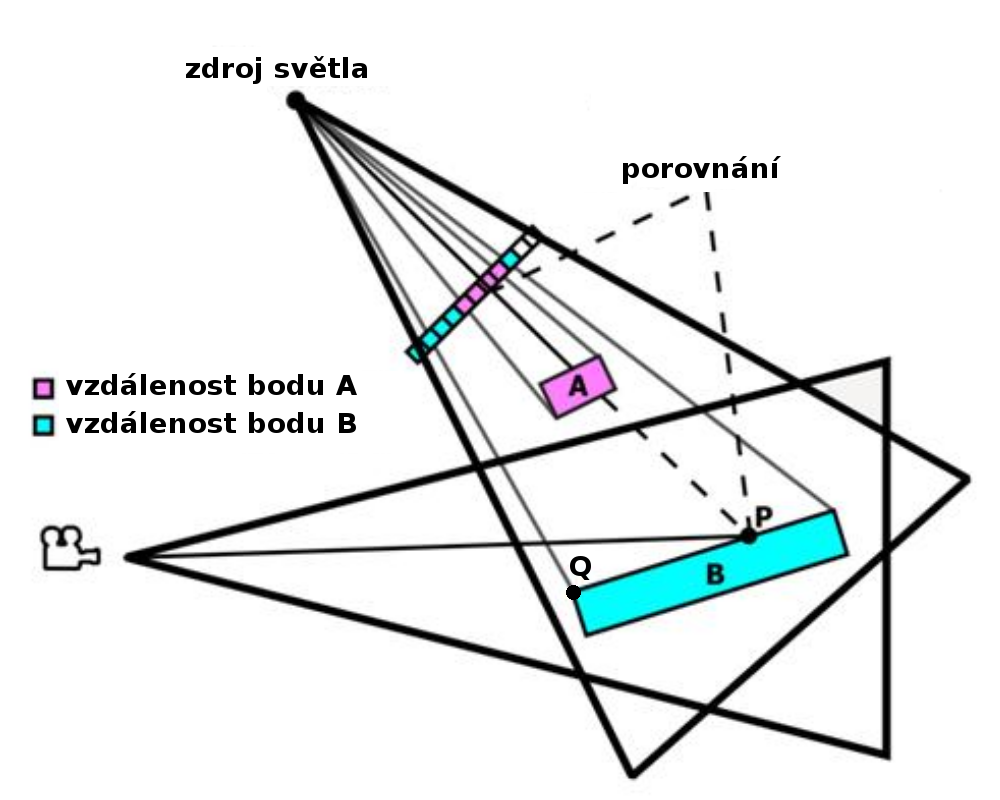
\includegraphics[width=90mm]{figures/shadowmaps.png}
\caption{Pomocný obrázek k výpočtu zastínění pomocí stínových map}
\end{figure}
\end{center}

\begin{center}
\begin{figure}[h]
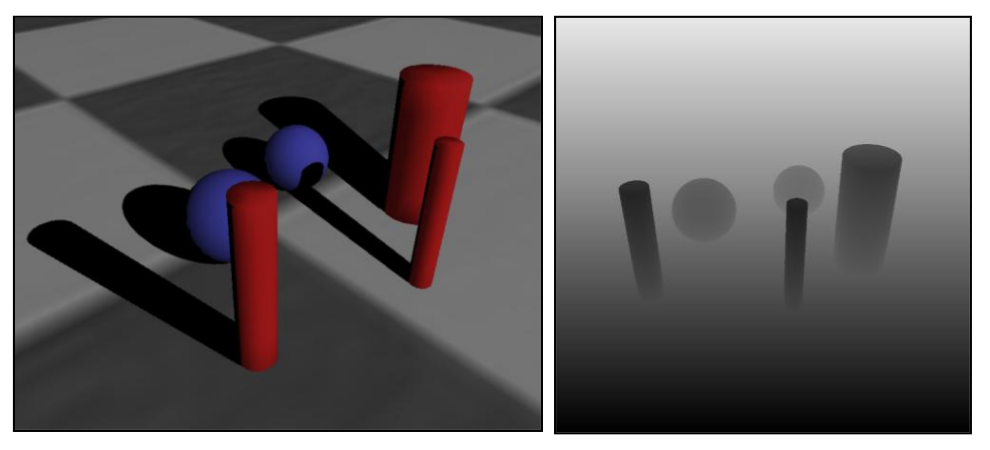
\includegraphics[width=120mm]{figures/shadowmap.png}
\caption{Ukázka scény (vlevo) a její stínové mapy (vpravo)}
\end{figure}
\end{center}

Transformace ze světových souřadnic do souřadnic projekce je vyjádřen pomocí součinu modelové, pohledové a projekční matice (anglicky model, view, projection matrix, používá se zkratka MVP). Transformaci kamery si označím jako $MVP_{camera}$ a transformaci pro pohled zdroje světla jako $MVP_{light}$. Vrchol primitiva si označím jako $\vec{v}$, spočteme vektor $\vec{p}$, jehož složky $x,y$ určují pozici hodnoty ve stínové mapě a složka $z$ hodnotu texelu. Pokud bychom měli hodnotu ve stínové mapě přepisovat, zapíšeme vždy nižší hodnotu (nižší hodnota je bod bližší zdroji světla).
\begin{center}
$\vec{p} = MVP_{light} \cdot \begin{pmatrix}\vec{v}\\ 1\\\end{pmatrix}$
\end{center}

Pomocí tohoto postupu získáme stínovou mapu, kterou využijeme při vykreslování scény z pohledu kamery. Vypočteme $\vec{p}$ stejně jako při výpočtu stínové mapy a získáme vzdálenost $d$ ze stínové mapy $SM$.
\begin{center}
$d = SM[\vec{p}_x, \vec{p}_y]$
\end{center}

Nakonec zjistíme, jak se tyto hodnoty liší pomocí podmínky $|\vec{p}_z - d| < \epsilon$, kde $\epsilon$ je malé číslo filtrující numerickou chybu. Pokud je podmínka splněna, je bod osvětlený daným zdrojem světla.
\bigskip

Výše uvedeným postupem jsou řešeny ostré stíny pro bodové zdroje světla, případně světelné reflektory. Dále je potřeba řešit měkké stíny, které vznikají z plošných zdrojů světla. Rozdíl mezi ostrými a měkkými stíny je znázorněn na obrázku 3.10.
\newpage

\begin{center}
\begin{figure}[h]
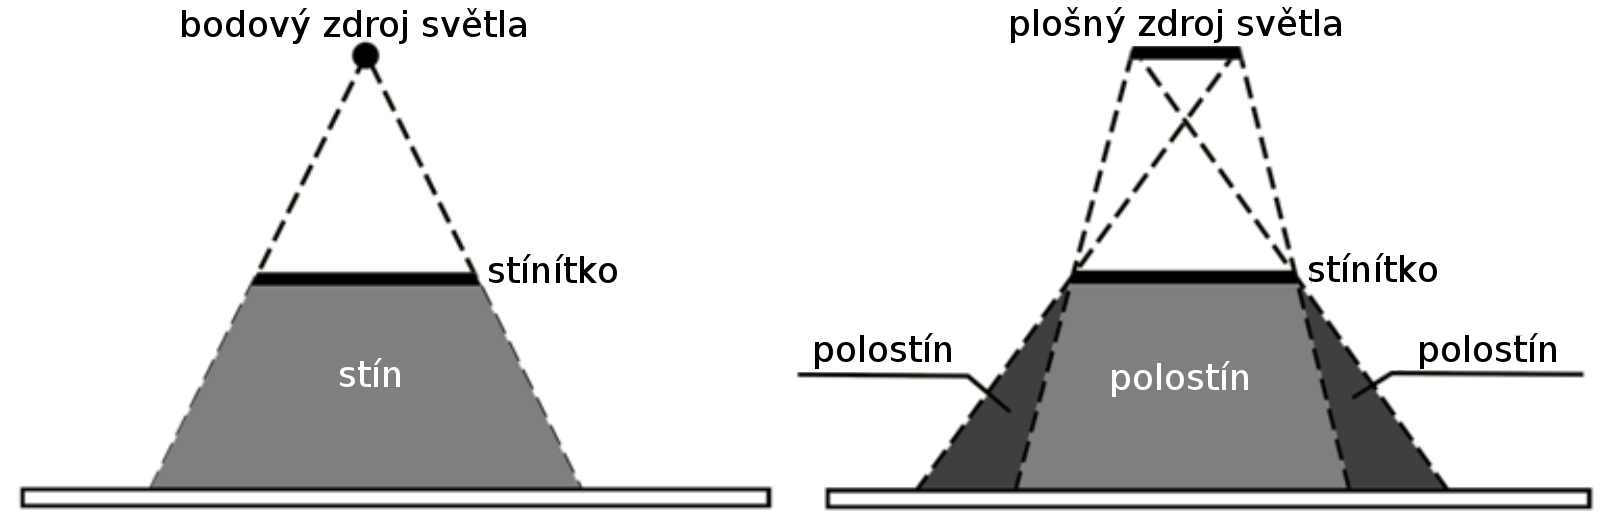
\includegraphics[width=110mm]{figures/shadows-pa.png}
\caption{Rozdíl mezi ostrými stíny (vlevo) a měkkými stíny (vpravo)}
\end{figure}
\end{center}

Výpočet plošných zdrojů světel v reálném čase je stále výpočetně příliš náročný. Pro zobrazení měkkých stínů je možné použít filtrování PCF (Percentage Closer Filtering), které umožní vytvořit měkký stín pro bodový zdroj světla.

Filtrování PCF je snadno implementovatelné, vrací dobré výsledky, ale může být náročnější na výpočetní výkon. Princip filtrování PCF je, že při výpočtu zastínění se ze stínové mapy vyhodnocují i okolní body a tím vzniká přechod mezi zastíněnými a nezastíněnými pixely na obrazovce.

\begin{center}
\begin{figure}[h]
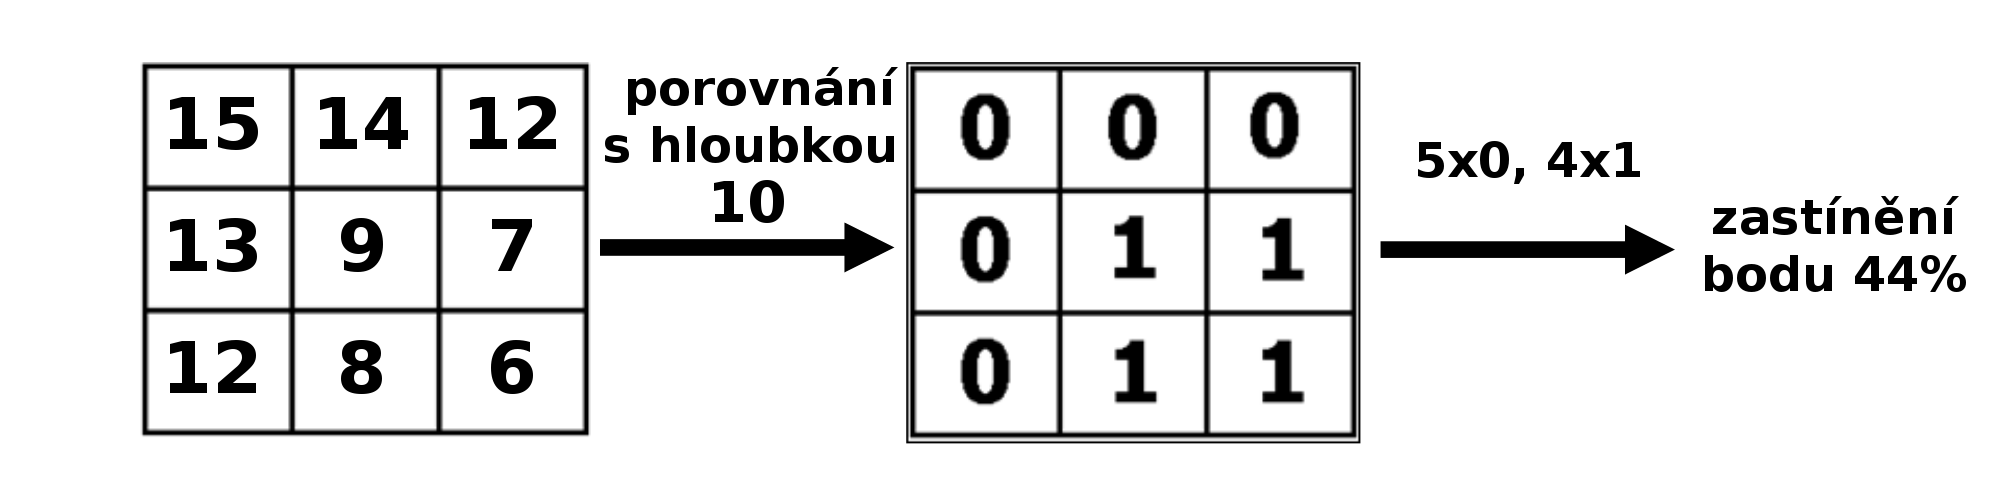
\includegraphics[width=85mm]{figures/pcf.png}
\caption{Ukázka vyhodnocení zastínění pomocí PCF 3x3. Vlevo jsou data ze stínové mapy, uprostřed vyhodnocení zastínění jednotlivých bodů (0 je viditelný bod, 1 je zastíněný bod) a vpravo výsledné zastínění}
\end{figure}
\end{center}

\begin{center}
\begin{figure}[h]
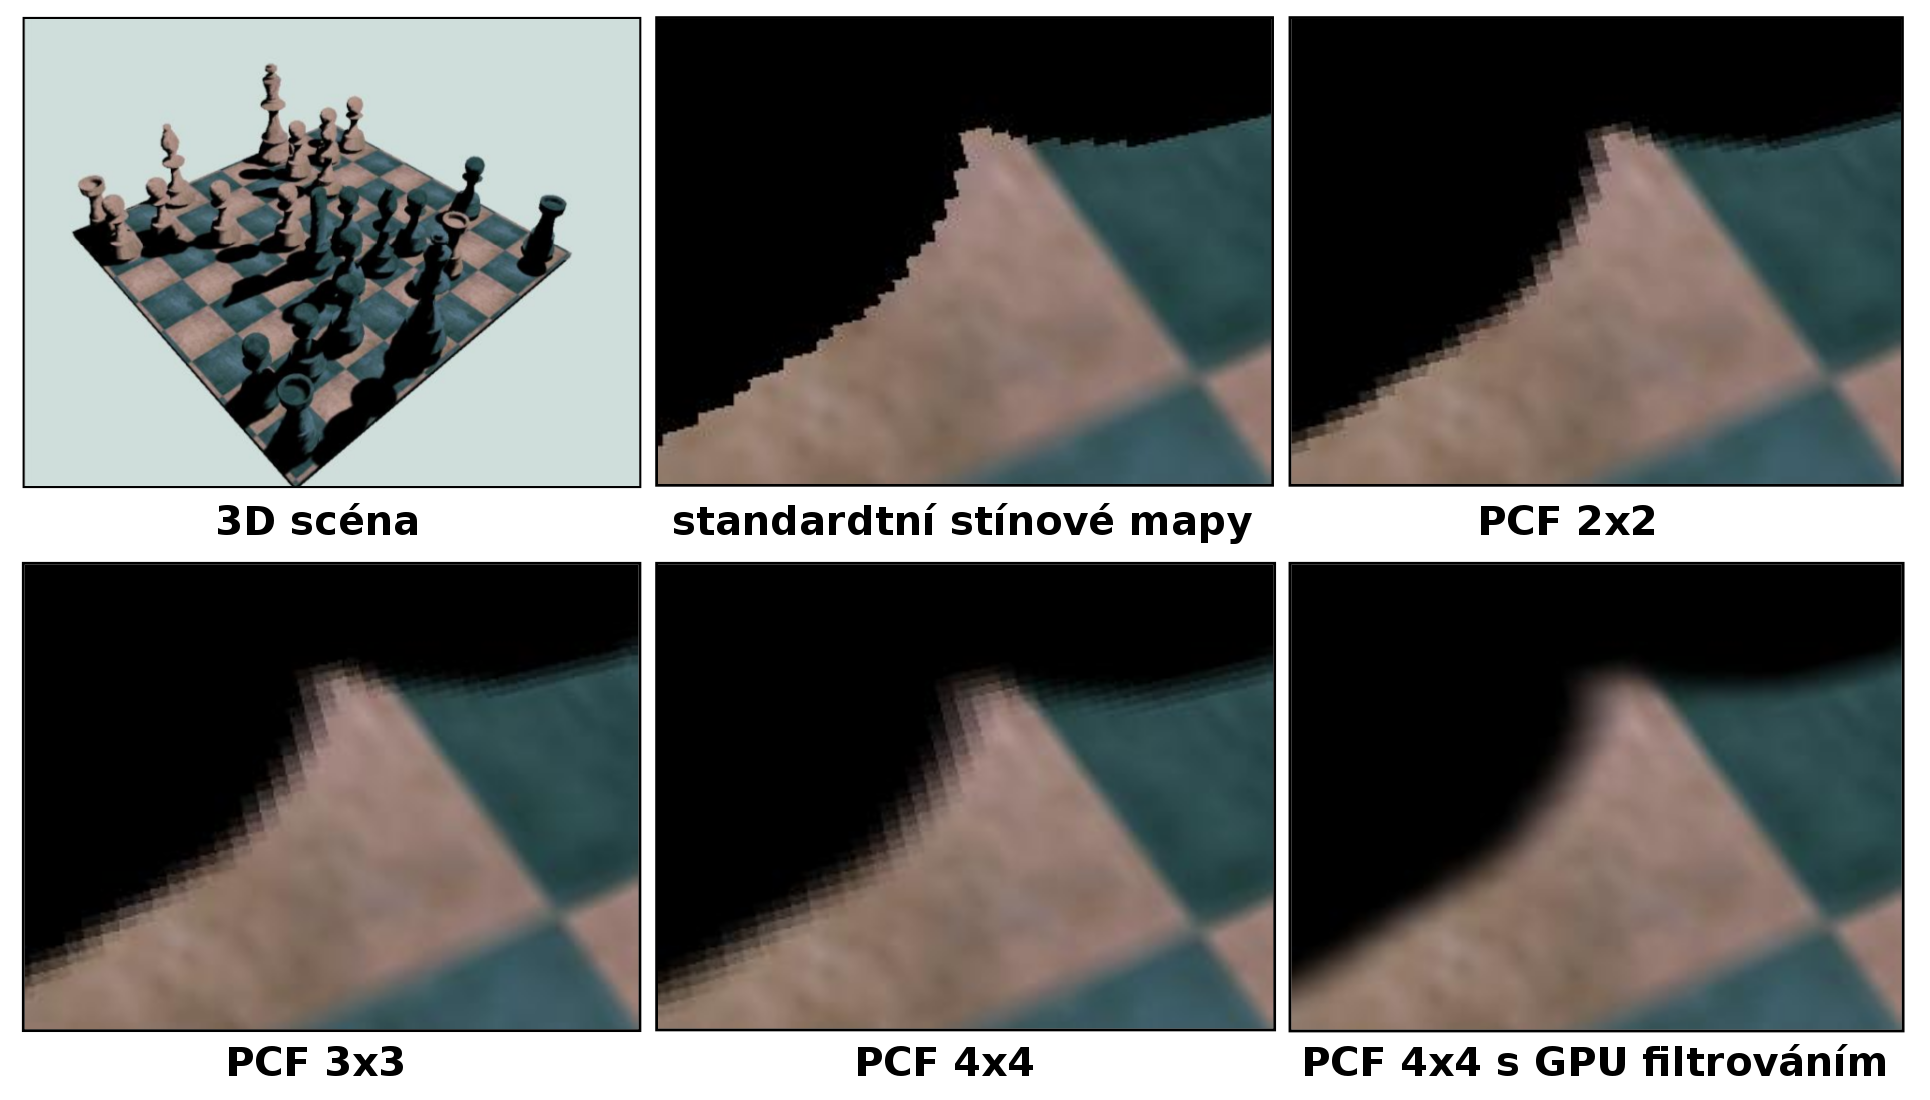
\includegraphics[width=100mm]{figures/pcf-example.png}
\caption{Ukázka výsledků filtrování PCF}
\end{figure}
\end{center}
\newpage

\section{Předpočtené osvětlení}
Předpočtené osvětlení je z hlediska vykreslování poměrně jednoduchá technika. Na 3D model se aplikuje další textura či textury, které mají vlastní texturovací souřadnice a nesou v sobě informaci o osvětlení jednotlivých trojúhelníků. Jak již bylo uvedeno, těmto texturám se říká mapy osvětlení a dalo by se říct, že se jedná o techniku, která rozšiřuje techniku předpočtených stínů.

Z hlediska generování těchto textur je tato technika náročnější než výsledné vykreslování, skládá se z několika kroků. V prvním kroku je třeba vytvořit texturovací souřadnice pro jednotlivé trojúhelníky.

\subsection{Vytvoření texturovacích souřadnic}
Pro mapy osvětlení není vhodné použít standardní texturovací souřadnice. V osvětlovacích mapách je potřeba zajistit, aby každý texel mapy odpovídal právě jednomu bodu\linebreak v prostoru. Pokud by tomu tak nebylo, stalo by se, že při osvětlení jednoho bodu se rozzáří\linebreak i jiný bod než ten osvětlený.

Obsah povrchu 3D modelu v ideálním případě odpovídá obsahu ploch map osvětlení. Abychom se tomuto případu přiblížili, musíme plochu map co nejvíce využít. Maximálním využitím 2D plochy se zabývá problém batohu, který patří do kategorie problémů NP-hard (obtížný nedeterministický problém řešitelný v polynomiálním čase).

Běžně se problém batohu zabývá pouze osově zarovnanými obálkovými tělesy (AABB). V této práci tento problém rozšiřuji o práci s trojúhelníky. Řešení spočívá ve spojování trojúhelníků do tvaru obdélníku, aby bylo možné problém řešit jako běžný problém batohu.

\begin{center}
\begin{figure}[h]
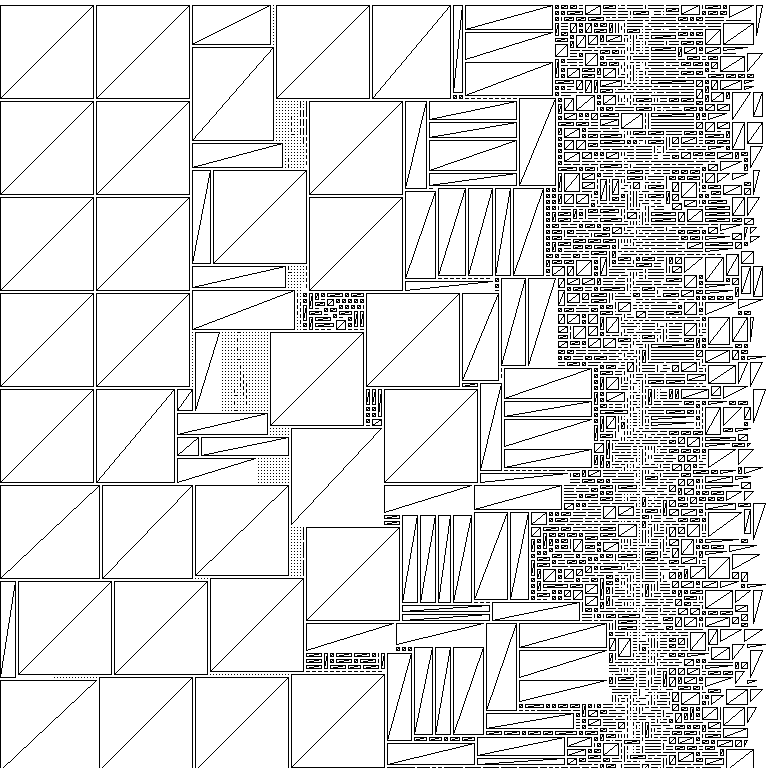
\includegraphics[width=80mm]{figures/lmcoords.png}
\caption{Výsledek řešení problému batohu se spárovanými trojúhelníky}
\end{figure}
\end{center}
\newpage

Problém batohu lze řešit pomocí ILP (Integer Linear programming). Problém lze přeformulovat pomocí kolizí dvou AABB. Pokud si všechny levé horní body AABB označím souřadnicemi $[minx, miny]$ a pravé dolní souřadnicemi $[maxx, maxy]$, platí poté následující výraz, pomocí kterého lze sestrojit ILP řešení (toto řešení neuvažuje otáčení AABB).

$\forall_{i,j}, i \neq j: (minx_i < maxx_j) \cap (miny_i < maxy_j) \cap (maxx_i > minx_j) \cap (maxy_i > miny_j)$
\bigskip

Abychom mohli problém řešit tímto způsobem, musíme mít nejdříve AABB místo trojúhelníků. Vytvoření AABB se zde provádí pomocí párování trojúhelníků. 

V prvním kroku se spočítá Eulerovská délka jednotlivých hran, nejdelší hranu označíme jako $c$ (to je přepona). Pokud chceme vytvořit plně využité AABB musíme mít všechny trojúhelníky pravoúhlé, z toho důvodu původní $c$ zahodíme a vytvoříme pravoúhlý trojúhelník o délce stran $a, b$. Pro novou přeponu platí $c' = \sqrt{a^2 + b^2}$.

\begin{center}
\begin{figure}[h]
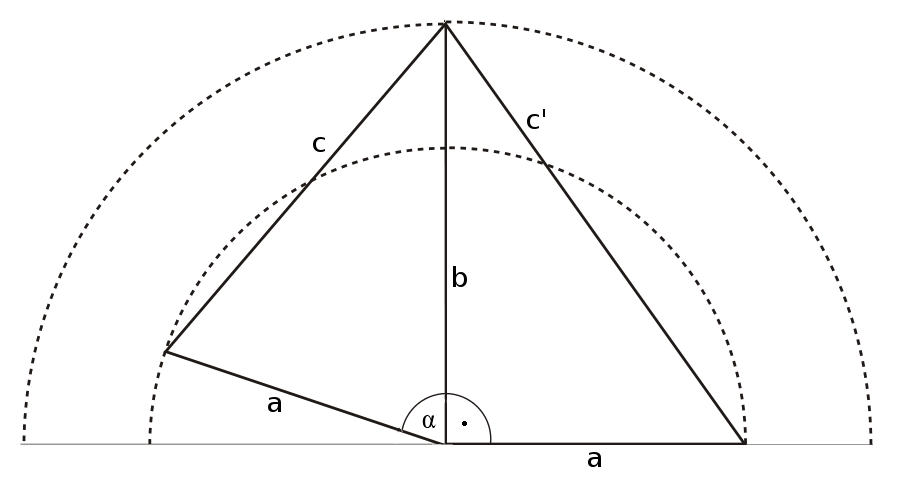
\includegraphics[width=100mm]{figures/triangle.png}
\caption{Změna délky přepony trojúhelníka pro vytvoření páru dvou trojúhelníků, vlevo původní nepravoúhlý trojúhelník, vpravo trojúhelník s novou délkou přepony}
\end{figure}
\end{center}

V dalším kroku hledáme párové trojúhelníky se stejnými délky stran $a, b$ (s určitou tolerancí), párové se spojí přeponou k sobě. Pro nepárové trojúhelníky vytvoříme AABB\linebreak o velikosti $a, b$ a tím máme vyřešený problém párování trojúhelníků.
\newpage

\subsection{Oprava chyby sousedících trojúhelníků}
Při použití výše uvedeného postupu vzniká problém při vykreslování, protože není\linebreak u texelů kolem přepon jednoznačné, ke kterému trojúhelníku texel patří a proto vznikají ve výsledné scéně artefakty. Stává se to, protože sousedící trojúhelníky v mapě osvětlení spolu nesousedí ve scéně.

\begin{center}
\begin{figure}[h]
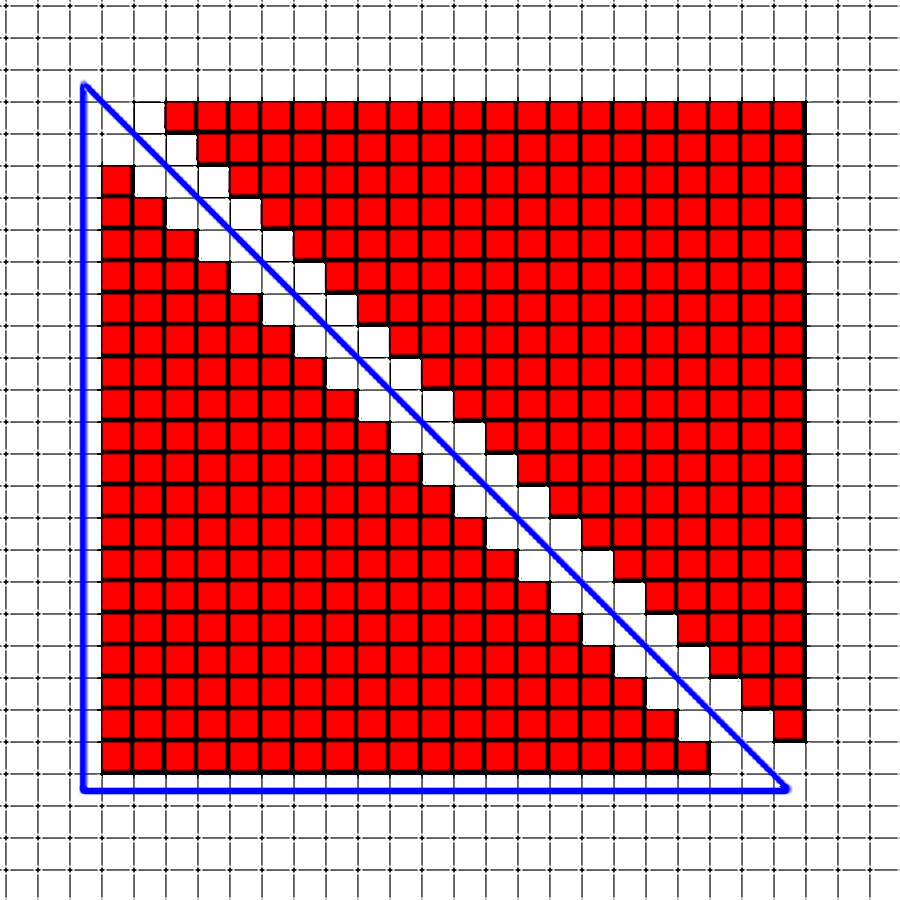
\includegraphics[width=60mm]{figures/lmfix.png}
\caption{Problém kolizních texelů dvou trojúhelníků}
\end{figure}
\end{center}

Provádí se zde posun texturovacích souřadnic směrem dovnitř trojúhelníku, aby k tomuto problému nedocházelo. Posouvají se i osově zarovnané hrany, protože při použití lineárního filtrování textur by docházelo k obdobným artefaktům jako v případě přepon.

\subsection{Generování map osvětlení}
Existují dvě základní metody generování map osvětlení, pomocí vrhání či sledování paprsku a pomocí rasterizace. V této kapitole popisuji rasterizační metodu (tedy pomocí OpenGL). Lze využít stínových map stejným způsobem, jako se používají k výpočtu zastínění v reálném čase. Rozdíl je pouze v transformování vrcholů a ve výpočtu barvy (nechceme vykreslovat texturu do světelných map, vedlo by to ke ztrátě kvality textur).

Nejdříve si vložíme ke každému vrcholu do VBO jeho souřadnice v osvětlovací mapě. Transformujeme vrchol do souřadnic mapy osvětlení. To se provede přiřazením souřadnic $u, v$ jako pozici ve FBO (s pozicí vrcholu se počítá pouze při výpočtu osvětlení).

Výslednou barvu texelu $C_t$ vypočteme z difúzního osvětlení pomocí níže uvedeného vzorce, kde $E_r$ je efektivita reflektoru, $F_a$ faktor útlumu, $C_l$ barva světla, $k_d$ koeficient difúzního odrazu, $\vec{L}$ je normalizovaný směr světla a $\vec{N}$ je normalizovaná normála povrchu. Více informací k výpočtu v kapitole 3.1.
\begin{center}
$C_t = E_r \cdot F_a \cdot C_l \cdot k_d \cdot (\vec{L} \cdot \vec{N})$
\end{center}

Pokud bychom chtěli použit i bodové zdroje světla, musíme mít stínovou mapu pro všechny možné směry světelných paprsků. K tomu lze využít tzv. cube mapování. Cube mapování je mapování scény na krychli, při kterém se na každou stěnu vykreslí pohled v jednom směru s perspektivním úhlem $90^{\circ}$. V případě využití cube mapování na stínové mapy, se pro každou stranu provádí výpočet jakoby se jednalo o samostatné světlo (efektivita reflektoru $E_r = 1$).

\begin{center}
\begin{figure}[h]
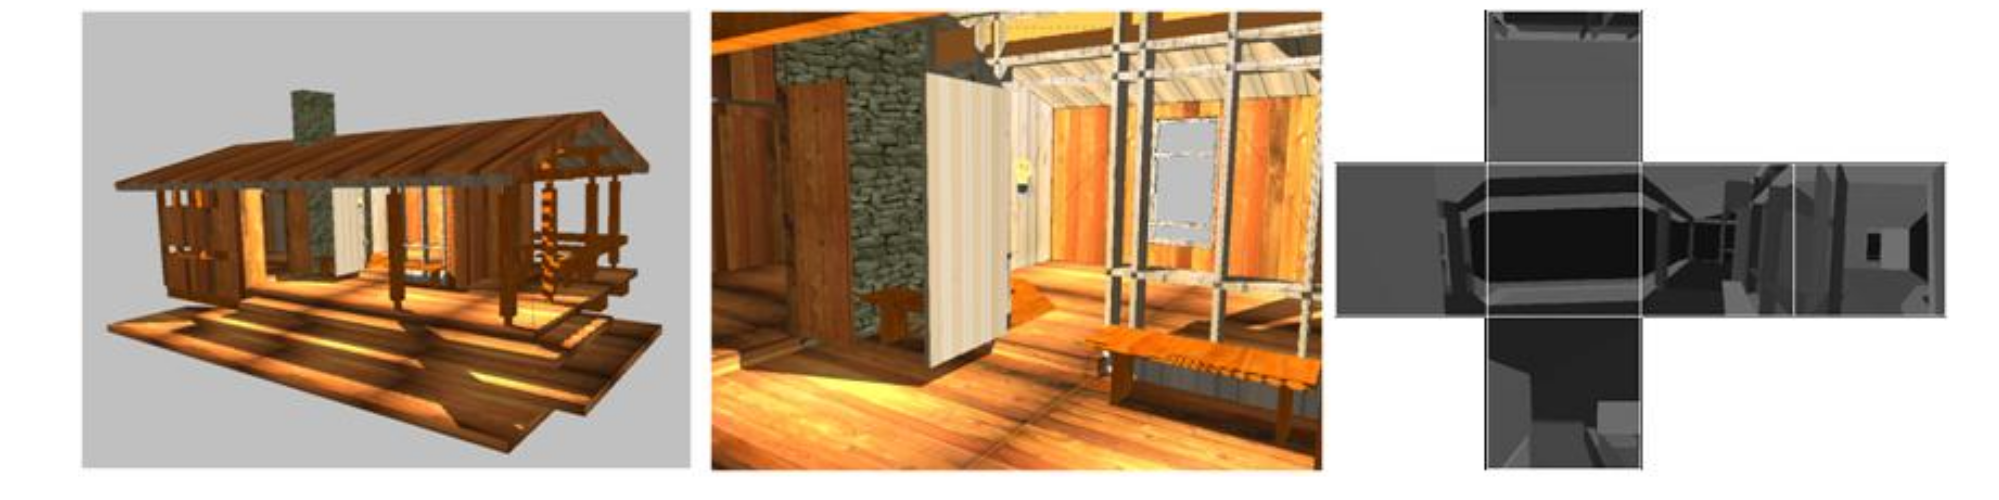
\includegraphics[width=150mm]{figures/cubemap.png}
\caption{Využití cube mapování na stínové mapy u bodových osvětlení, vlevo dva náhledy scény, vpravo stínová mapa}
\end{figure}
\end{center}

\subsection{Spekulární složka osvětlovací modelu}
Spekulární složka osvětlovacího modelu je závislá na pohledu kamery a nelze jí tedy předpočítat a také nelze počítat v reálném čase spekulární složky pro desítky světel. Tento problém se dá řešit vypnutím vzdálených světel. Světla se seřadí podle vzdálenosti\linebreak od kamery a provede se započítání $n$ nejbližších (konstantu $n$ je vhodné mít co nejnižší, protože spekulární složka je poměrně náročná na výpočet). 

Nutno podotknout, že tento přístup neřeší viditelnost světla. Stejný přístup lze použít\linebreak i pro difúzní osvětlení, ale předpočtené osvětlení je efektivnější.

\section{Odlesky povrchů}
Odlesky dodávají scéně lepší vzhled, dodávají dojem buď kovového nebo mokrého povrchu. V rasterizačním řetězci jsou odlesky drobet problematické, protože grafická karta vždy zpracovává pouze aktuální geometrii a nemá informace o okolí.

Standardně se odlesk realizuje dalším průchodem, ve kterém se vykreslí okolí do textury\linebreak a tato textura se poté aplikuje na model s odleskem. U menších objektů, jako je například auto, se vykreslí okolí pomocí cube mapování do FBO. Výsledná textura se následně namapuje na objekt a tím se získá dojem lesklého povrchu.
\newpage

V případě rovných povrchů je nutné použít jiný přístup, scéna se vykreslí do textury\linebreak z pohledu pod povrchem, který je na obrázku 3.17 označen jako $P'$. Pohled snímá objekty jakoby z povrchu a při vykreslování na obrazovku se spočítá pozice daného pixelu povrchu ve vykreslené textuře a z té se aplikuje barva pixelu.

\begin{figure}[h!]
\begin{center}
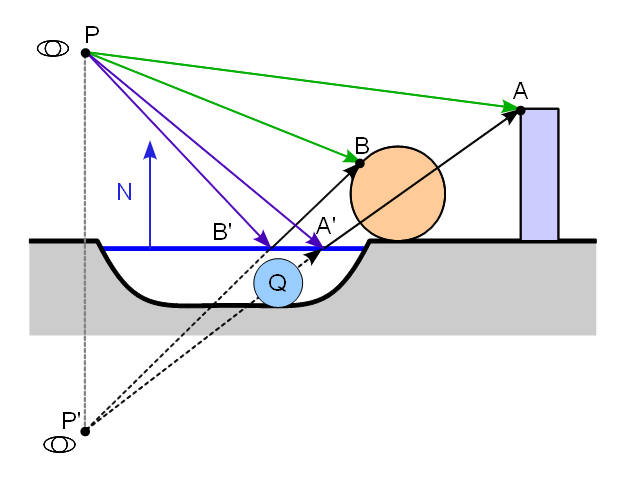
\includegraphics[width=80mm]{figures/reflection-diagram.png}
\caption{Diagram odrazu vodní hladiny \cite{Kaplinski11}}
\end{center}
\end{figure}

Pohled $P$ je MVP matice, pro získání pohledu $P'$ potřebujeme vypočítat reflexní matici $R$, která převrátí pohled podle normály povrchu $\vec{N}$ a parametru $d$ spočítaného z rovnice roviny.
              
\begin{center}
$d = -(xN_x + yN_y + zN_z)$
\end{center}
\begin{center}
$R = \begin{pmatrix}
1 -2 \cdot {\vec{N}_x}^2 & -2 \cdot \vec{N}_x \cdot \vec{N}_y & -2 \cdot \vec{N}_x \cdot \vec{N}_z & -2 \cdot \vec{N}_x \cdot d\\
-2 \cdot \vec{N}_y \cdot \vec{N}_x & 1 -2 \cdot {\vec{N}_y}^2 & -2 \cdot \vec{N}_y \cdot \vec{N}_z & -2 \cdot \vec{N}_y \cdot d\\
-2 \cdot \vec{N}_z \cdot \vec{N}_x & -2 \cdot \vec{N}_z \cdot \vec{N}_y & 1 -2 \cdot {\vec{N}_z}^2 & -2 \cdot \vec{N}_z \cdot d\\
0 & 0 & 0 & 1
\end{pmatrix}$
\end{center}

Vynásobením matice $R$ s maticí $P$ získáme reflekční matici, která otáčí obraz o $180^{\circ}$, abychom získali korektní pohled, musíme provést ještě rotaci kolem osy Z.
\begin{center}
$P' = R \cdot P \cdot \begin{pmatrix}
-1 & 0 & 0 & 0\\
0 & -1 & 0 & 0\\
0 & 0 & 1 & 0\\
0 & 0 & 0 & 1
\end{pmatrix}$
\end{center}

Při vykreslování reflexního pohledu je nutné provést ořez scény pod povrchem a nevykreslovat odvrácené trojúhelníky. Pro finální vykreslování si označím reflexní mapu jako $RM$ a vykreslovaný vrchol jako $\vec{v}$. Barva odlesku $color_r$ se spočítá dle níže uvedeného vzorce.
\begin{center}
$\vec{p} = P' \cdot \begin{pmatrix}
\vec{v}\\
1
\end{pmatrix}$
\end{center}
\begin{center}
$color_r = RM[\vec{p}_x, \vec{p}_y]$
\end{center}


%*****************************************************************************
\chapter{Realizace}
Realizace projektu byla provedena ve třech fázích. Nejdříve byla vytvořena verze pro PC bez předpočteného osvětlení, dále bylo provedeno portování projektu na Android\linebreak a v poslední fázi jsem se zabýval předpočteným osvětlením a problémy s ním spojené.

\section{Simulátor}
Simulátor je navržen tak, aby fungoval na X11-Linuxu a Androidu. Znamená to výběr multiplatformních knihoven nebo ve výjimečných případech rozdílných implementací pro jednotlivé platformy. K vykreslování jsem vybral OpenGL ES 2.0 (jedná se o odlehčené OpenGL 3.0) a GLSL core verzi 1.0 (to zaručuje maximální možnou kompatibilitu).

Fyzikální vlastnosti vozidel jsou realizovány pomocí enginu Bullet Physics (tento engine používá mnoho známých firem zabývajících se vývojem mobilních her). Zvuk je realizován na mobilních zařízeních pomocí Android API a na Linuxu pomocí knihovny FMOD API. Správce oken je na Androidu třeba doprogramovat, aby fungovalo dotykové ovládání a pozastavení simulátoru (např. při hovoru). Na Linuxu je použitá knihovna freeglut.

Samotný simulátor je rozdělen do dvou oddělených částí. První část je abstraktní\linebreak a řeší logickou část projektu. Abstrakce je realizována pomocí rozhraní, které definují společné metody abstraktních objektů. Druhá část implementuje jednotlivá rozhraní a řeší také načítání dat ze souborů.
\lstset{language=C++} 
\begin{lstlisting}[caption=Načtení 3D modelu vozidla pomocí abstraktního přístupu]
    /// load models
    skin = getModel(getConfigStr("skin_model", atributes), false);
    wheel = getModel(getConfigStr("wheel_model", atributes), false);

    /// set car wheels position
    wheelX = getConfig("wheel_x", atributes);
    wheelY = getConfig("wheel_y", atributes);
    wheelZ1 = getConfig("wheel_back", atributes);
    wheelZ2 = getConfig("wheel_front", atributes);
\end{lstlisting}
\newpage

Důvodem oddělení částí je, že implementace jednotlivých rozhraní může být v budoucnu snadno nahrazena anebo mohou být použité různé implementace pro různé platformy. Příkladem různých implementací rozhraní pro různé platformy může být například renderer.\linebreak V simulátoru je využita knihovna OpenGL, která například na platformě Windows Phone není dostupná a bylo by potřeba na této platformě použit Direct3D.

\begin{figure}[h]
\begin{center}
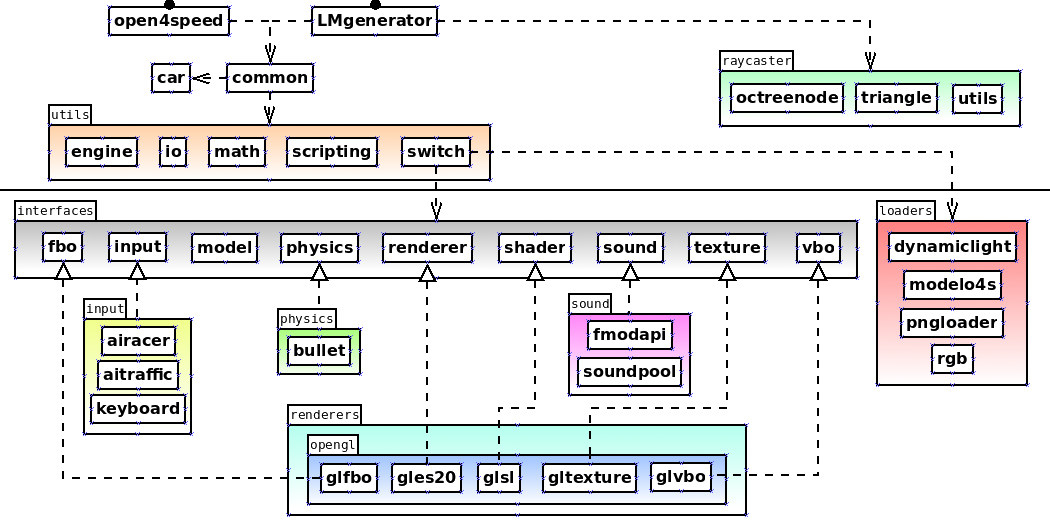
\includegraphics[width=160mm]{figures/o4suml.png}
\caption{UML diagram projektu, horní část je abstraktní, dolní část implementuje jednotlivá rozhraní a načítá data do paměti, spustitelné soubory jsou označeny tečkou}
\end{center}
\end{figure}
Jak je vidět na obrázku 4.1, simulátor je rozdělen do dalších dílčích částí. Část \ul{raycaster} a třída \ul{LMgenerator} realizují předzpracování. Třída \ul{open4speed} se zabývá správou okna\linebreak a spouštění dílčích součástí. \ul{Common} uchovává veškeré objekty a proměnné, je to z důvodu, že jinak by v třídách \ul{open4speed} a \ul{LMgenerator} musel být obsah struktury \ul{common} duplicitně.

Třída \ul{car} je v první řadě struktura uchovávající veškeré proměnné realizující vozidlo, dále zajišťuje propojení mezi fyzikálním enginem, vykreslováním, zvukem, vstupem umělé inteligence a uživatele.
\\ \\
Část \ul{utils} je balík příkazů tvořící simulátor.
\begin{itemize}
\item \ul{engine} realizuje GUI a 3D scénu
\item \ul{io} obstarává práci se soubory
\item \ul{math} poskytuje sadu matematických příkazů pro práci s 3D objekty
\item \ul{scripting} interpretuje skriptování GUI
\item \ul{switch} obstarává objekty jednotlivých rozhraní a naplňuje je daty
\end{itemize}

Jednotlivá rozhraní mají různé funkce. Rozhraní \ul{fbo}, \ul{renderer}, \ul{shader}, \ul{texture} a \ul{vbo} vytváří abstraktní přístup k OpenGL, \ul{input} je rozhraní pro ovládání vozidla (implementací může být buď klávesnice anebo umělá inteligence), rozhraní \ul{physics} reprezentuje fyzikální engine a rozhraní \ul{sound} umožňuje přehrávat zvuky. Implementace rozhraní \ul{sound} jsou příkladem použití různých implementací na různých platformách.

\section{Realizace na platformě Android}
Platforma Android je postavená na Linuxovém jádře a využívá mnohé komponenty\linebreak z projektu GNU, nicméně celé Android API je v jazyku Java za využiti virtuálního stroje Dalwik. Pomocí Android NDK(native development kit) je možné zkompilovat C/C++ kód jako knihovnu, kterou je možné zavolat z jazyku Java. Toto je prováděno pomocí JNI(Java native interface).

Snažší by bylo naprogramovat simulátor přímo v Javě, ale tím bych ztratil možnost portovat simulátor na další platformy, které virtuální stroj Dalwik nemají. Dále by byl problém s použitím fyzikálního enginu, který je napsaný v jazyce C++. Musel bych napsat interface pro fyzikální engine, který by mi umožnil komunikaci mezi C++ a Java kódem.

\subsection{Problematika Android API}
Java native interface je rozhraní, které umožňuje spustit C++ kód z jazyku Java a obráceně. Největší problém je, že neexistuje použitelný port freeglut knihovny pro Android. Udělal jsem tedy JNI rozhraní, které odpovídá handlerům knihovny freeglut. Tedy nahrazuji veškeré funkce této knihovny svou implementací. Knihovna implementuje správu oken, vstup klávesnice a myši a volání idle a display funkcí. Klávesnice a myš byla pochopitelně plně nahrazena dotykovým ovládáním, ale pokud do Android zařízení připojíme klávesnici nebo myš, bude plně funkční. Funkčnost myši zařizuje sám systém, klávesnice stačila namapovat.

Aby bylo možné volat C++ metody přímo z Javy musí být pojmenovány ve formátu Java\_\textit{package}\_\textit{třída}\_\textit{metoda}. C++ knihovna bude tedy možné spustit pouze z jedné Java třídy.
\lstset{language=C++} 
\begin{lstlisting}[caption=JNI metody v C++ kódu pro nahrazení freeglut knihovny]
extern "C" {
  void Java_com_cvut_o4s_O4SJNI_nativeInit(JNIEnv* e, jstring apkPath ) {
    instance = env;
    APKArchive = zip_open(env->GetStringUTFChars(apkPath), 0, NULL);
    main(0, 0);
  }
  void Java_com_cvut_o4s_O4SJNI_nativeClick(JNIEnv* e, jint x, jint y) { 
    mouseClick(0, 0, x, y); 
  }
  void Java_com_cvut_o4s_O4SJNI_nativeKey(JNIEnv* e, jint i) { keyDown(i); }
  void Java_com_cvut_o4s_O4SJNI_nativeKeyUp(JNIEnv* e, jint i) { keyUp(i); }
  void Java_com_cvut_o4s_O4SJNI_nativeDisplay(JNIEnv* e) { display(); }
  void Java_com_cvut_o4s_O4SJNI_nativeLoop(JNIEnv* e) { idle(0); }
}
\end{lstlisting}

Dále je potřeba C++ knihovnu načíst pomocí volání System.loadLibrary a metody deklarovat v dané Java třídě pomocí klíčového slova native.

\lstset{language=Java} 
\begin{lstlisting}[caption=Deklarování C++ metod v Java kódu]
package com.cvut.o4s;

class O4SJNI {

  static { System.loadLibrary("open4speed"); }
  static native void nativeInit(String apkPath);
  static native void nativeClick(int x, int y);
  static native void nativeKey(int i);
  static native void nativeKeyUp(int i);
  static native void nativeDisplay();
  static native void nativeLoop();

  ...
}
\end{lstlisting}

Dalším problémem je volání Android API z C++ kódu (tzn. volání Java kódu z C++). Příkladem je přehrávání zvuků pomocí Android API, ovládání zvuku je nutno řídit z C++, kdežto API je přímo přístupné pouze z Javy. Na obrázku 4.2 je to případ třídy Sounds. Problém se řeší také pomocí JNI, pouze volání jsou prováděny v opačném směru.

\begin{center}
\begin{figure}[h]
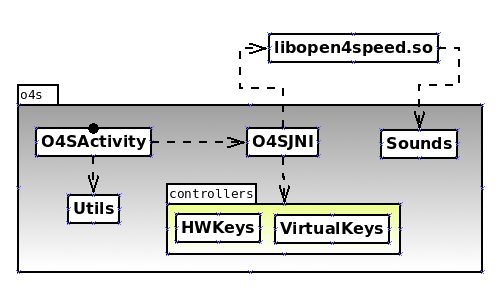
\includegraphics[width=80mm]{figures/jni.png}
\caption{UML diagram spustitelného klienta pro Android, kde libopen4speed.so je zkompilovaná C++ knihovna projektu}
\end{figure}
\end{center}

\lstset{language=C++} 
\begin{lstlisting}[caption=Volání Java metody pro přehrání zvuku z C++ kódu]
void soundpool::play(int index) {
  jclass clazz = instance->FindClass("com/cvut/o4s/Sounds");
  //get method "void soundPlay(int, int)"
  jmethodID method = instance->GetStaticMethodID(clazz, "soundPlay", "(II)V");
  instance->CallStaticVoidMethod(clazz, method, index, (int)looping);
}
\end{lstlisting}
\newpage

V Javě se poté musí ještě rozlišovat přehrávání zvuků od přehrávání hudby. Hudba bývá řádově náročnější na paměť a nemá smysl jí celou držet v paměti, když na ni není potřeba aplikovat další zvukové efekty.

\lstset{language=Java} 
\begin{lstlisting}[caption=Přehrání zvuku v Javě pomocí Android API]
package com.cvut.o4s;

import ...

class Sounds {
  // instances of sounds
  static ArrayList<Sound> list;
  // instances of sound APIs
  static MediaPlayer music;
  static SoundPool snd;
  
  ...  
  
  public static void soundPlay(int index, int loop) {
    //instance is a music
    if (list.get(index).id == TYPE_MUSIC) {
      music.setLooping(loop == 1);
      music.start();
    }

    //audio clip
    else {
      Sound s = list.get(index);
      snd.play(s.id, s.volume, s.volume, 1, loop, s.rate);
    }
  }
}
\end{lstlisting}

\subsection{Využití vláken}
Většina zařízení, které dnes už spadají do střední třídy, je vybavena aspoň dvěma procesory, je proto vhodné rozdělit činnost do více vláken, aby bylo dosaženo maximálního výkonu. Třída GLSurfaceView, která umožňuje vykreslovat OpenGL scénu z C++ umožňuje volat OpenGL příkazy pouze z jednoho vlákna. Z tohoto důvodu jsem rozdělil kód na grafické\linebreak a negrafické vlákno.

V menu simulátoru se používá pouze grafické vlákno, negrafické vlákno je primárně použito pro fyzikální výpočty, které zařízení vytěžují nejvíce. Vlákna jsou synchronizovaná, aby nedocházelo k použití transformace vozidla z předešlého snímku(to by bylo velmi rušivé).

Dále provádím regulaci rychlosti simulátoru v závislosti na výkonu hardwaru. Je potřeba, aby obě vlákna prováděla výpočet co nejvíce paralelně, pokud by negrafické vlákno příliš dlouho nedodávalo novou transformaci vozidla, docházelo by k trhanému vykreslování (některý snímek by se vykresloval víckrát a to by se projevilo tak, že by se snímková frekvence zdála být na krátký okamžik poloviční). Pokud k tomuto případu dojde, je vhodné snížit frekvenci volání obou vláken a tím snížit rychlost simulátoru.

Problém je, že nelze snižovat rychlost simulátoru do nekonečna, proto je zde nastavena minimální hodnota, na kterou se může simulátor zpomalit. Je zde i horní limit, aby nedocházelo k zrychlené jízdě a tedy i ke zvýšené spotřebě energie.

\subsection{Práce se soubory}
V Androidu se aplikace publikují v APK balíčku. Jedná se o ZIP soubor, který má nějakou danou strukturu. V Java kódu je možné na veškeré soubory uvnitř balíčku přistupovat,\linebreak v C++ tato možnost není. Někteří vývojáři toto řeší, že po prvním spuštění si aplikace stáhne ze serveru přídavná data a ty si uloží například na paměťovou kartu. Lze také rozbalit soubory z APK balíčku a s těmi pak v C++ pracovat. To se moc nepoužívá, protože jsou potom data v zařízení dvakrát.

Další možnou variantou je přistupovat k APK balíčku jako k ZIP souboru. Knihovna libZIP umožňuje zpracovávat data ze ZIP souboru jako kdyby byla uložena normálně na disku nebo na paměťové kartě. To má výhodu, že data jsou komprimovaná a zároveň přístupná.
\lstset{language=C++} 
\begin{lstlisting}[caption=Čtení řádky z APK balíčku (vlevo) a ze souboru (vpravo)]
void gets(char* line, zip_file* f) {   |  void gets(char* line, FILE* f) {
  for (int i=0; i<MAX_LENGTH; i++) {   |    for (int i=0; i<MAX_LENGTH; i++) {
    zip_fread(f, character, 1);        |      fread(character, 1, 1, f);
    line[i] = character[0];            |      line[i] = character[0];
    if (line[i] == '\n') {             |      if (line[i] == '\n') {
      line[i + 1] = '\000';            |        line[i + 1] = '\000';
      return;                          |        return;
    }                                  |      }  
  }                                    |    }      
}                                      |  }   
\end{lstlisting}

Problém může nastat při použití externích knihoven, které čtou ze souborů. To je případ knihovny libPNG, která načítá ze souborů PNG rastrová data. Tato knihovna umožňuje použití vlastní čtecí funkce a tím umožňuje číst data přímo z APK, kdyby tomu tak nebylo, nemohli bychom touto knihovnou načítat data přímo z APK balíčku.

\lstset{language=C++} 
\begin{lstlisting}[caption=Použití vlastní čtecí funkce při použití knihovny libPNG]
void png_read(png_structp png_ptr, png_bytep data, png_size_t length) {
#ifdef USE_APK_PACKAGE
  zip_fread(zipFile, data, length);
#else
  fread(data, length, 1, file);
#endif
}

Texture* loadPNG(const char* filename) {
#ifdef USE_APK_PACKAGE
  zipFile = zip_fopen(APKArchive, prefix(filename), 0);
#else
  file = fopen(prefix(filename), "rb");
#endif
  png_set_read_fn(png_ptr, NULL, png_read);
  ...
}
\end{lstlisting}

\section{Předpočtené osvětlení}
Předpočtené osvětlení umožňuje velmi rychle zobrazovat stínování a stíny na statických objektech. Problémem je, že je potřeba aplikovat tento efekt i na dynamických objektech. Úroveň osvětlení lze přečíst z nejbližšího statického objektu, tedy za předpokladu, že budeme mít tuto hodnotu někde k dispozici. Tuto hodnotu lze mít uloženou v alfa kanálu aktuálního snímku a jen jí přečíst před tím, než se vykreslí dynamické objekty.

\begin{figure}[h!]
\begin{center}
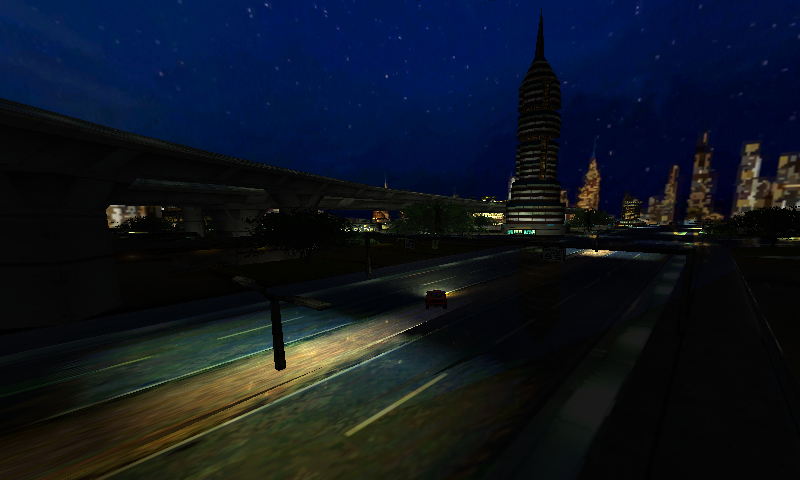
\includegraphics[width=120mm]{figures/lamps.png}
\caption{Scéna s aplikovanými mapami osvětlení lamp}
\end{center}
\end{figure}

\subsection{Vytváření map osvětlení}
Vytváření map osvětlení je realizováno dvěma přístupy, první je rasterizační (pomocí OpenGL) a druhý je vrhání paprsku. Pro rasterizační přistup jsou k dispozici dva druhy světel: bodové světlo a reflektor. Tyto světla jsou definovaná přímo v 3D modelovacím software. Dosah světel je omezen na 300metrů (je to z důvodu chyb, které vznikají u osvětlení\linebreak na velkou vzdálenost). Světla pochopitelně nepoužívají spekulární složku, protože tato složka je závislá na pohledu kamery a tudíž jí nelze předpočítat.

I maximální možné rozlišení map osvětlení pro použitou scénu není dostatečné a stíny jsou kostičkované. Z tohoto důvodu se používají dva druhy filtrování. Prvním je rozmazání map osvětlení, které se provádí přímo po generování mapy osvětlení a druhým je lineární filtrování, které se aplikuje až při aplikování mapy osvětlení. Tato kombinace filtrování značně zvýší výslednou kvalitu stínů.

V přístupu využívající vrhání paprsku jsou navíc k dispozici plošné zdroje světla, které jsou definovány pomocí osvětlovacích textur, což jsou textury, u kterých jsou vykresleny pouze texely vyzařující světlo. Osvětlovací textury mají stejné texturovací souřadnice jako difúzní textury 3D modelu. Plošný zdroj světla se realizuje tak, že každý barevný texel\linebreak v osvětlovací textuře vygeneruje bodový zdroj světla. Množina vzniklých bodových světel pak tvoří plošný zdroj světla.

\begin{figure}[h]
\begin{center}$
\begin{array}{cc}
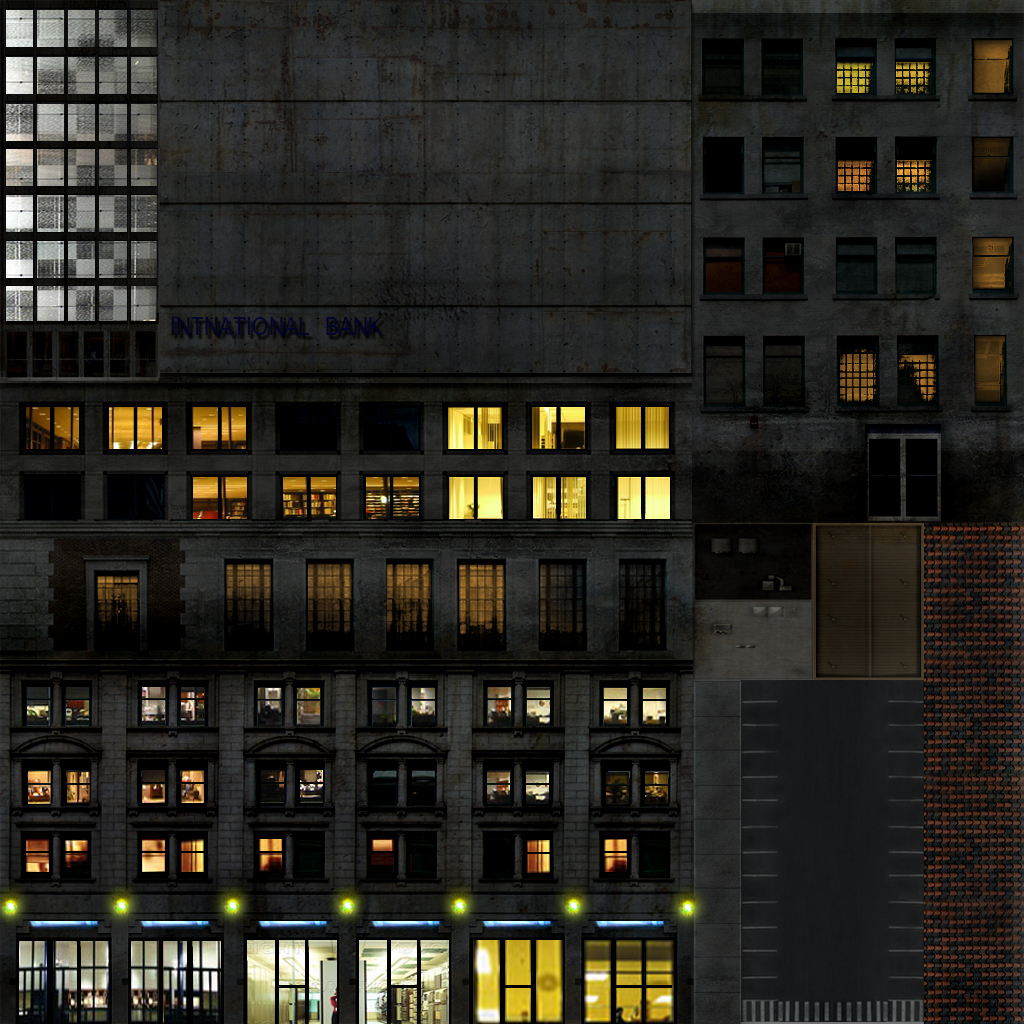
\includegraphics[width=50mm]{figures/buildz3-n.png} &
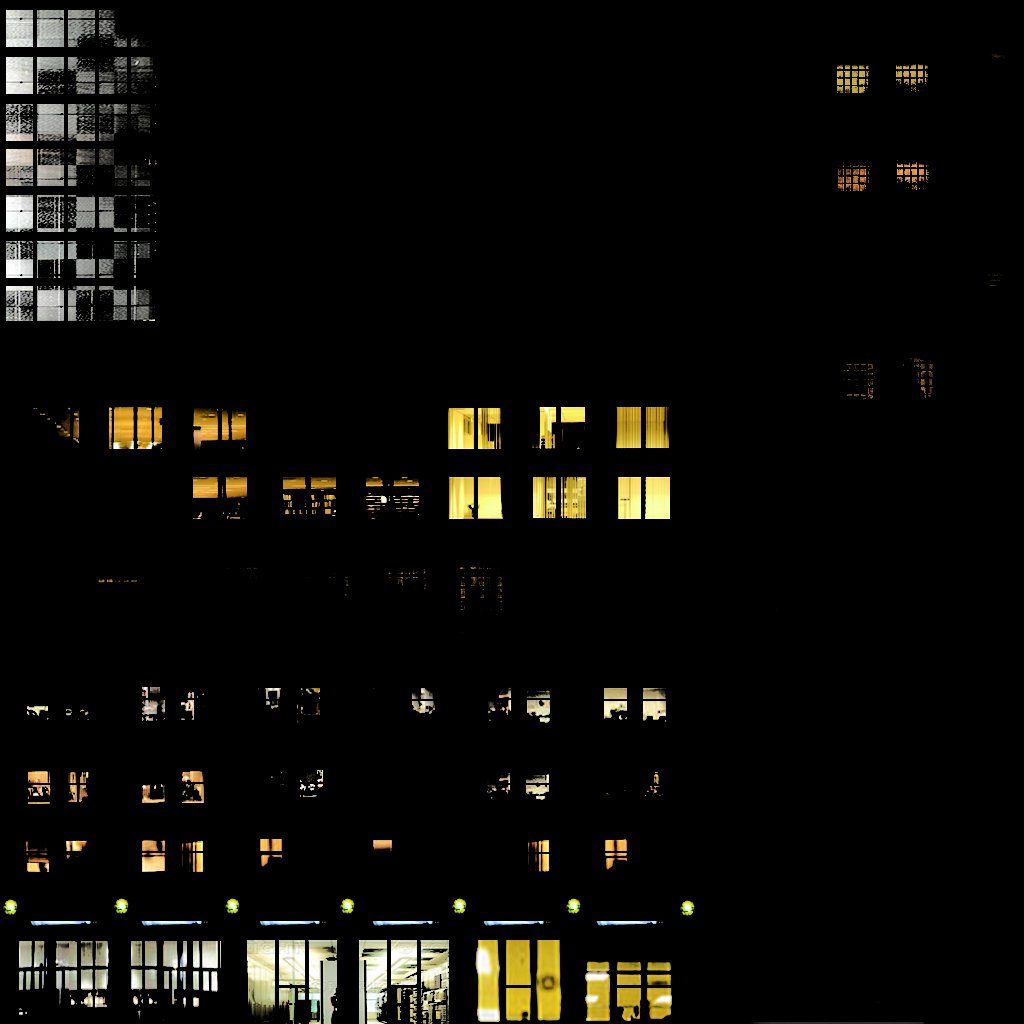
\includegraphics[width=50mm]{figures/buildz3-e.png}
\end{array}$
\end{center}
\caption{Ukázka difúzní textury modelu (vlevo) a osvětlovací textury (vpravo)}
\end{figure}

\subsubsection{Generování texturovacích souřadnic pro mapy osvětlení}
V teoretické části byl popsán postup generování texturovacích souřadnic pomocí ILP.\linebreak V praxi toto řešení nelze použít, protože jeho výpočetní složitost $f(m, n)$ $\epsilon$ $O(m^2 \cdot n^2)$, $m$ je počet trojúhelníků a $n$ počet texelů v lightmapě.  Pomocí ILP se tedy dají řešit pouze velice malé instance problému. V této práci problém řeším pomocí metody Packing Lightmaps, což je metoda řešící problém batohu za použití datové struktury kD stromu, která dělí $k$-rozměrný objekt půlením.

V případě Packing Lightmaps dělíme rovinu horizontálním nebo vertikálním řezem, kD strom je v podstatě binární strom, jehož kořen reprezentuje k-rozměrný objekt (v našem případě mapu osvětlení). Vnitřní uzly jsou dělící, určují podle které osy se řez povede a je v nich zapsána pozice řezu. Listy stromu reprezentují objekty uložené ve struktuře, v této práci AABB - tedy dva párové trojúhelníky (viz kapitola 3.6.1).

\begin{center}
\begin{figure}[h]
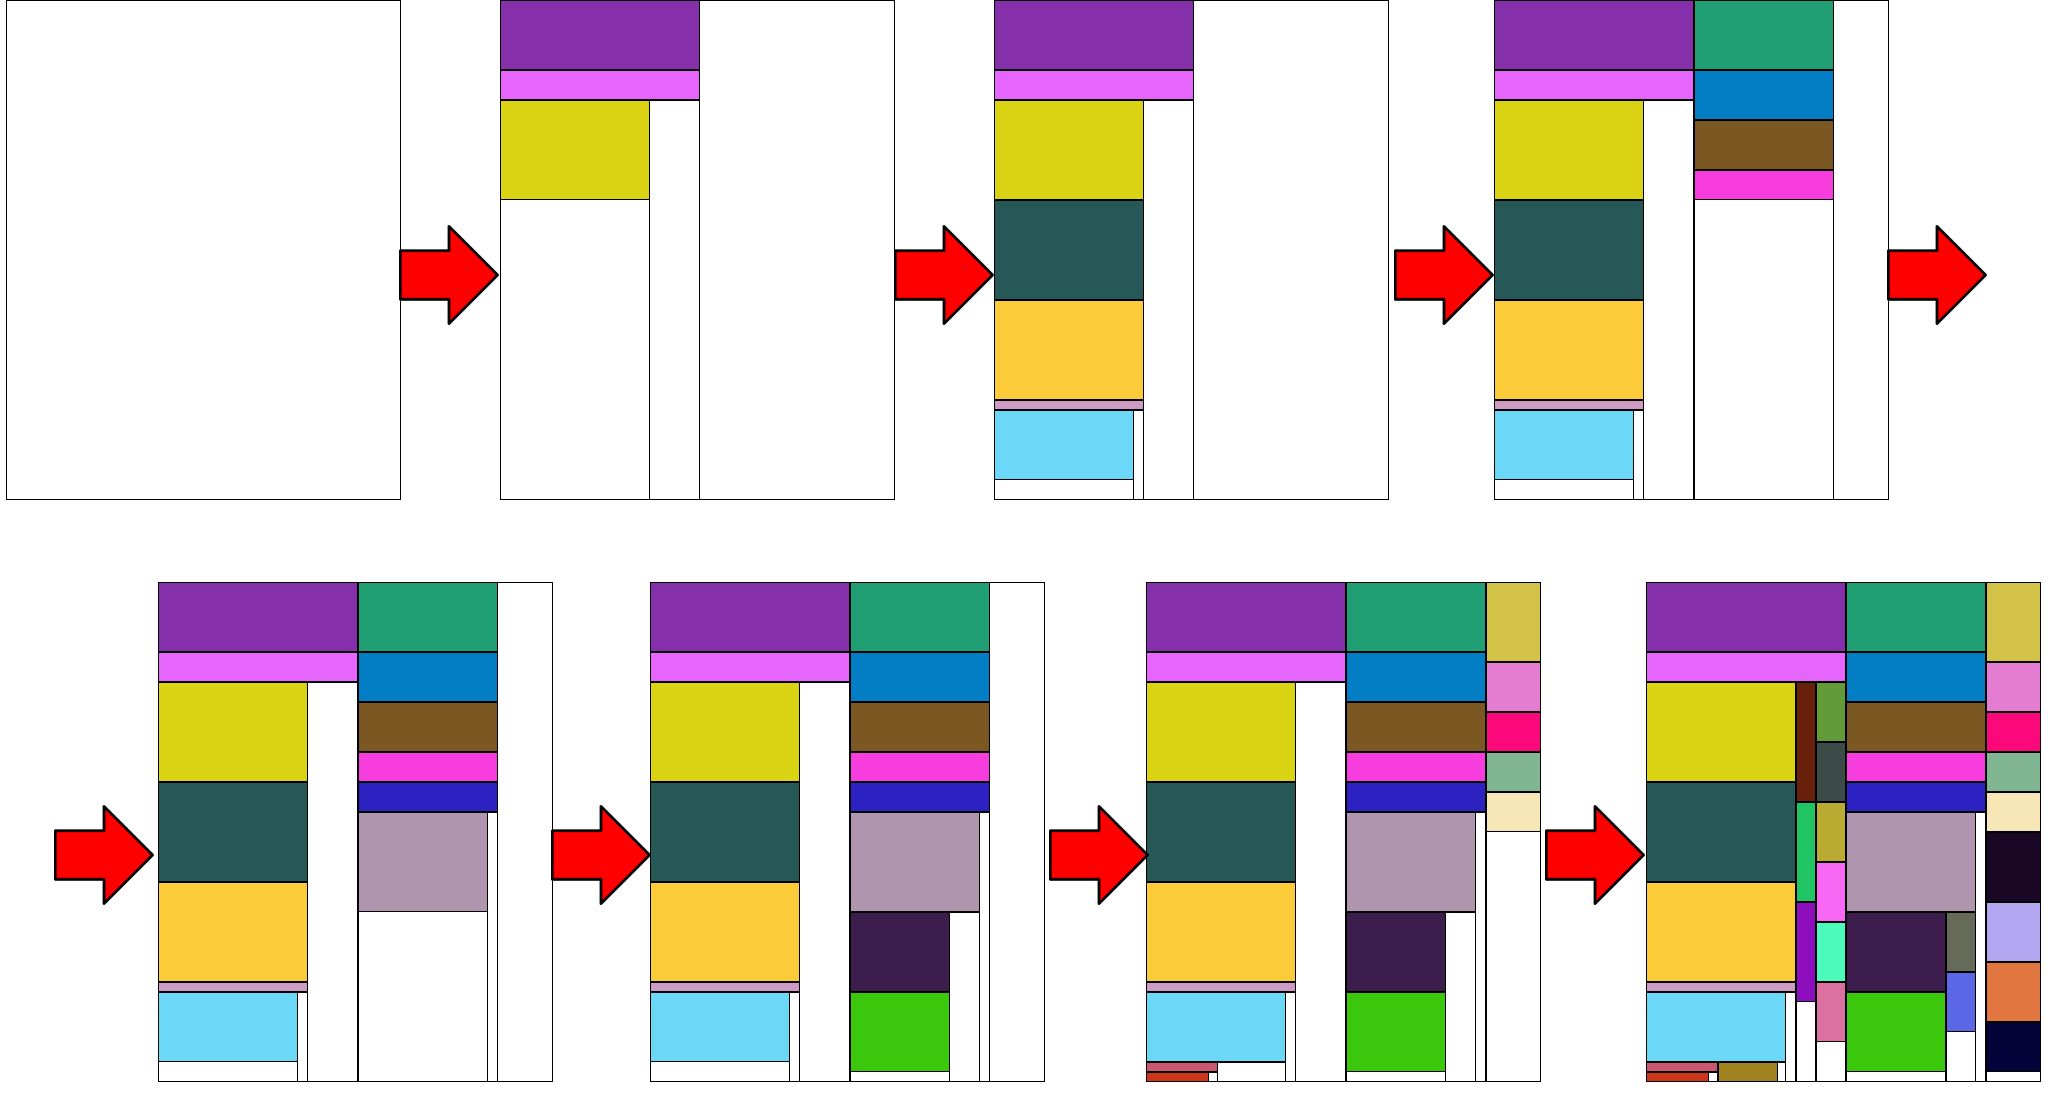
\includegraphics[width=120mm]{figures/kd.png}
\caption{Ukázka naplnění kD stromu pomocí metody Packing Lightmaps}
\end{figure}
\end{center}

Metoda Packing Lightmaps nejdříve seřadí AABB podle jejich plochy a postupně je vkládá do kD stromu. Při každém vložení se nejdříve hledají neobsazené listy, zda neexistuje takový, který by odpovídal rozměrům AABB. Pokud takový neexistuje pokusí se algoritmus nalézt takový neobsazený list, kterému odpovídá aspoň jeden rozměr. V případě úspěšného hledání se AABB vloží do listu, v ostatních případech se najde větší list, provede se jeho rozdělení a následně se AABB do jednoho z potomků vloží.

\lstset{language=Java} 
\begin{lstlisting}[caption=Vkládání AABB do kD stromu za využití rekurze]
public boolean addAABB(AABB aabb) {
  // check if current node is empty and has enought space for AABB
  if (isEmpty() && (aabb.width <= width) && (aabb.height <= height)) {

    // fits exactly
    if ((aabb.width == width) && (aabb.height == height)) {
      child1 = new KDNode(aabb);
      return true;
    } 
        
    // subdivision
    else {
      child1 = new KDNode(aabb.width, height);
      if (child1.addAABB(aabb))
        return true;
    }
  } 
    
  // try to insert into first child
  else if (child1.addAABB(aabb))
    return true;

  // create second child
  else if (child2 == null) {
    
    // horizontal subdivision
    if ((aabb.width <= width) && (aabb.height <= getChild2Height())) {
      child2 = new KDNode(width, height - aabb.height);
      if (child2.addAABB(aabb))
        return true;
    }
      
    // vertical subdivision
    if ((aabb.width <= getChild2Width()) && (aabb.height <= height)) {
      child2 = new KDNode(width - child1.width, height);
      if (child2.addAABB(aabb))
        return true;
    }
  } 
    
  // try to insert into second child
  else if (child2.addAABB(aabb))
    return true;
  return false;
}
\end{lstlisting}

\subsubsection{Generování map osvětlení}

\subsection{Příprava dat pro dynamickou aktualizaci map osvětlení}

\subsection{Dynamické osvětlení a dynamické objekty}

\subsection{Světla vozidel}

Dle předběžných měření jsem zjistil, že na mobilních zařízeních lze za běhu počítat jedno až dvě světla(bez řešení viditelnosti světla). U vozidla ovládané hráčem není potřeba řešit viditelnost světla, prakticky zde nedochází k situacím, že by světlo osvětlovalo neviditelné objekty(je to z důvodu těsné vazby světlo hráčova vozidla-kamera).

U ostatních vozidel je třeba osvětlení zjednodušit, aby to mobilní hardware zvládal. Zvolil jsem metodu vykreslování kuželů do scény. Při vykreslování je použita OpenGL funkce blending, která umožňuje kreslit objekty s částečnou průhledností. Dále je také zapnuté ořezávání odvrácených trojúhelníku. Střed kužele je vyplněn několikrát zevnitř s odvrácenou normálou. Z toho důvodu je osvětlení silnější pokud světlo svítí do kamery než od kamery.

\section{Nahrazení víceprůchodových přístupů}
Při běhu jakéhokoliv simulátoru je největší zátěž mobilního hardware způsobena vykreslováním 3D scény, proto je nutné tuto část co nejvíce zefektivnit. Pro mnoho efektů se používají takzvané víceprůchodové přístupy(scéna se vykreslí víckrát z různých pohledů nebo pomocí různých shaderů), ale na mobilním zařízení je zatím z hlediska výkonu možné použít pouze jednoprůchodový přístup.

Abych částečně nahradil ve svém simulátoru víceprůchodový přístup, použil jsem screen-space přístup(to je obecně jakákoliv technika využívající data z pohledu kamery, jinými slovy máme pouze výsledný snímek a na něm provádíme další operace). V praxi se používá hlavně pro zrcadlové plochy. Potřeboval jsem přistupovat do aktuálně vykreslovaného snímku. To je ale problém, protože tento snímek není kompletní a kdybych vykresloval přímo do něj\linebreak a zároveň z něj četl způsobilo by to chyby ve výsledném obraze.

Řešením je vykreslování střídavě do dvou různých textur. To znamená, že při lichém snímku kreslím do textury 1 a čtu z textury 2. Při sudém snímku je tomu obráceně. Tímto způsobem získám přístup do vykreslené scény, sice s drobným zpožděním, ale při dostatečně rychlém vykreslování si toho uživatel nevšimne(za předpokladu, že textura bude použita\linebreak na efekty jako jsou odlesky nebo stíny).

\begin{figure}[h!]
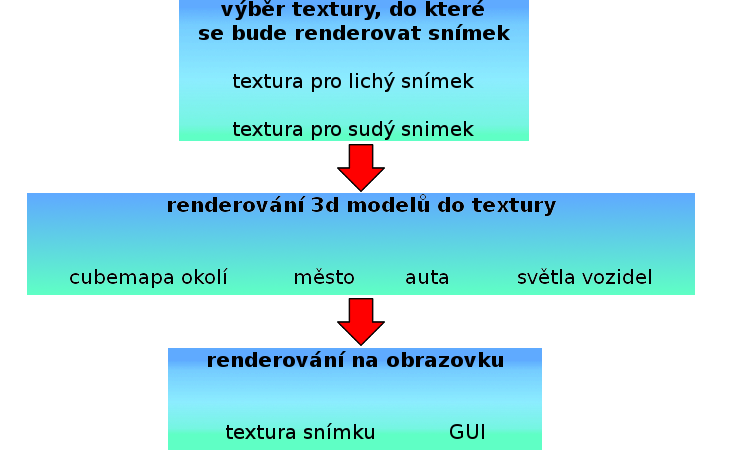
\includegraphics[width=150mm]{figures/render-schema.png}
\caption{Vykreslovací řetězec simulátoru}
\end{figure}

\subsection{Rozměr textur na OpenGL ES 2.0}
Verze OpenGL ES 2.0 neumožňuje používat obdélníkové textury. Textury musí být čtvercové a jejich strana musí být o velikosti mocniny 2.
Pro vykreslování do textury, která bude výsledně umístěna na obrazovku je tedy nutné zvolit vyšší rozlišení. Např. u tabletu Google Nexus 7 2012 s rozlišením 1280x720 se zvolí textura 2048x1024. To znamená, že by se ve výsledku vykreslilo víc než 2x více pixelů než je potřeba.

Není ale nutné vykreslovat do celé textury, pomocí příkazu \textit{glViewport} se dá nastavit část textury, do které má OpenGL vykreslovat a nedojde tedy k plýtvání výkonem(bude se plýtvat pouze pamětí).

Dále je možné zvolit nižší rozlišení viewportu než je rozlišení displeje. Mobilní zařízení obvykle disponují obrovskou hustotou pixelů a pokud zařízení nebude stíhat vykreslovat scénu v plném rozlišení, lze vykreslovat v rozlišení menším. U počítačových 3D her se také setkáváme s možností změnit rozlišení, tam řeší změnu přímo hardware displeje nebo jeho ovladač.

\subsection{Odlesky}

Jedním z velmi rychlých efektů ve screen-space je \textbf{motion-blur}.
\lstset{language=GLSL} 
\begin{lstlisting}[caption=Motion blur fragment shader dle rychlosti vozidla]
uniform sampler2D color_texture, pFrm;
uniform float res, speed;
varying vec2 v_Coords;

void main() {
	//apply color texture
	gl_FragColor = texture2D(color_texture, v_Coords); 

	//apply motion blur
	gl_FragColor *= (1.0 - speed);
	gl_FragColor += speed * texture2D(pFrm, gl_FragCoord.xy * res);
}
\end{lstlisting}

Speed je rychlost vozidla od 0 do 1, pFrm je textura předchozího snímku a res je 1 / plné rozlišení textury(pro jednoduchost je použitý čtvercový rozměr textury).

Tento kód je použit přímo při renderování modelů, nikoliv při postprocesu. Výhodou je, že rozmaznutí se projeví po několik snímků za sebou pomocí jednoho čtení textury navíc. Nevýhodou je, že tento kód musí být vložen do každého shaderu vykreslující 3D model.
\bigskip

Dále je možné ve screen-space řešit \textbf{odlesky}. Existuje obecný(složitý) postup jak tyto odlesky vypočítat, který by mobilní hardware nezvládl. Problém jsem rozdělil podle typu ploch. Vzhledem k tomu, že v simulátoru dochází pouze k rotaci pohledu podle osy y(rotace yaw), je možné řešit pro odlesky pro různé směry normál zvlášť.

Například u vozovky stačí nalézt, kde vozovka končí, a podle toho obraz převrátit. Korektně to pro zatím z hlediska výkonu není možné vypočítat, proto dochází k velké nepřesnosti odlesku. Odhad zlomu je prováděn pomocí normály a pozice daného fragmentu, do kterého se odlesk započítává.

\begin{figure}[h!]
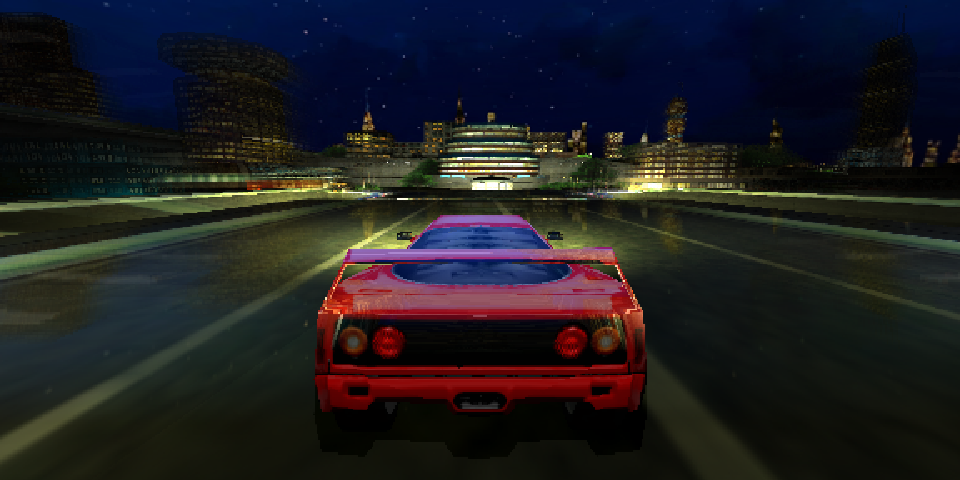
\includegraphics[width=150mm]{figures/reflect-horizont.png}
\caption{Odlesky na povrchu vozovky.}
\end{figure}
\bigskip

U vozidel se odlesk provádí pouze podle normály. Pro výpočet pozice odraženého obrazu se vezme střed vozidla a přičte se k němu normála vynásobena určitým faktorem(funguje pouze u vozidla, které uživatel ovládá).

\begin{figure}[h!]
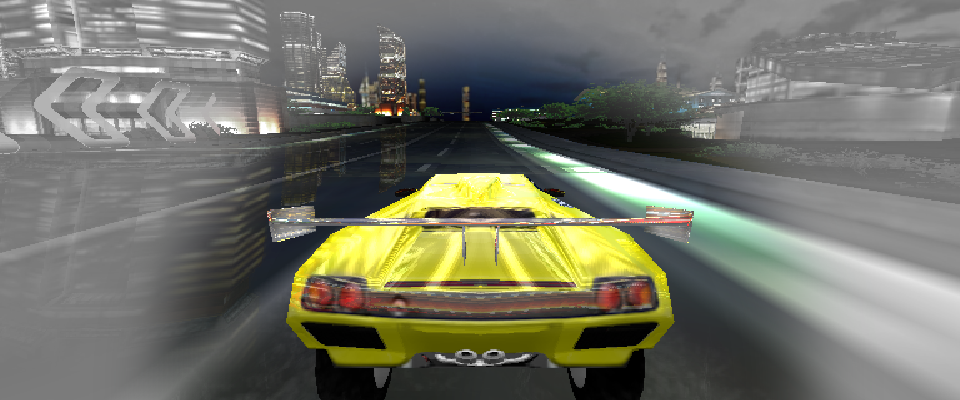
\includegraphics[width=150mm]{figures/reflect-car.png}
\caption{Odlesky na vozidle. Bílé plochy znázorňují pozice, ze kterých se čte barva odlesku.}
\end{figure}
\newpage

Pokud máme ve scéně \textbf{předpočtené stíny}, je vhodné tyto statické stíny aplikovat\linebreak i \textbf{na dynamické objekty}. V případě vozidla lze přečíst intenzitu osvětlení z některých bodů na silnici pod vozidlem. Intenzitu osvětlení lze jednoduše ukládat do alfa kanálu textury,\linebreak ve které se nachází aktuální scéna.

Zde vzniká problém s barevným světlem. Jsou zde dvě možnosti řešení. Prvním je přidání další textury, ve kterém by byla barevná intenzita světla(tím by došlo ke zvýšení náročnosti na hardware a ke zvýšení paměťové náročnosti). Druhým možným řešením je omezit barevná světla do nějaké sytosti(pokud se slabě zabarvené světlo aplikuje jako bílé, není to tolik rušivé).

%*****************************************************************************
\chapter{Testování}
Testování probíhalo na smartphonu, tabletu a laptopu, které jsou blíže popsány v tabulce 5.1. Zařízení byla během testování plně nabita, byla připojena ke zdroji napájení a byly vypnuty volby úspory energie. Veškeré testy byly prováděny v režimu \uv{free ride} a za stejných podmínek.

\begin{table}[h!]
\begin{center}
\begin{tabular}{|p{35mm}|p{35mm}|p{35mm}|p{35mm}|}
\hline
& \textbf{Samsung Galaxy S3 mini (mobil)} & \textbf{Google Nexus 7 2012 (tablet)} & \textbf{Acer TravelMate P253-e (laptop)} \\
\hline
Procesor & NovaThor U8500 & ARM Cortex-A9 & Intel 1005M \\ \hline
Počet jader & 2 & 4+1* & 2 \\ \hline
Frekvence CPU & 1.0GHz & 1.3GHz & 2.4GHz \\ \hline
Operační paměť & 1GB & 1GB & 4GB \\ \hline
Grafická karta & ARM Mali-400 MP & Nvidia Tegra 3 & Intel HD Graphics \\ \hline
Rozlišení displeje & 800x480 & 1280x800 & 1366x768 \\ \hline
Operační systém & Android 4.1 & Android 4.4 & Kubuntu 13.10 32bit \\ \hline
\end{tabular}
\caption{Parametry zařízení, na kterých jsem projekt testoval}
*tablet má extra procesor pro nižší spotřebu během nečinnosti
\end{center}
\end{table}
\newpage

\section{Generování map osvětlení}
\paragraph{Bodové zdroje světla}\ \ \\
\begin{table}[h!]
\begin{center}
\begin{tabular}{|p{50mm}|c|}
\hline
\textbf{Nastavení} & \textbf{Čas vykreslování} \\
\hline
OpenGL bez PCF & 2.25min\\ \hline
OpenGL s PCF8x8 & 19.267min\\ \hline
raycasting & 28.176min\\ \hline
\end{tabular}
\caption{Vykreslování 106 bodových zdrojů světla pomocí OpenGL a pomocí raycastingu}
\end{center}
\end{table}

\paragraph{Plošné zdroje světla}\ \ \\
\begin{table}[h!]
\begin{center}
\begin{tabular}{|p{100mm}|c|}
\hline
\textbf{Nastavení} & \textbf{Čas vykreslování} \\
\hline
kvadratický útlum 0.2, optimalizováno & 10.276s\\ \hline
kvadratický útlum 0.1, optimalizováno & 19.483s\\ \hline
kvadratický útlum 0.05, optimalizováno & 36.875s\\ \hline
kvadratický útlum 0.05, neoptimalizováno & 359.796s\\ \hline
lineární útlum 0.05, neoptimalizováno & 960.546s\\ \hline
lineární útlum 0.05, spot effekt 0.5, neoptimalizováno & 12874.661s\\ \hline
\end{tabular}
\caption{Vykreslování několika plošných zdrojů světel navzorkovaných na 202 bodových světel, optimalizace spočívá v testování paprsků vždy mezi dvěma trojúhelníky a detekování, zda bod na trojúhelník dosvítí }
\end{center}
\end{table}

\begin{table}[h!]
\begin{center}
\begin{tabular}{|p{100mm}|c|}
\hline
\textbf{Nastavení} & \textbf{Čas vykreslování} \\
\hline
kvadratický útlum 0.1, optimalizováno & 4.925h\\ \hline
kvadratický útlum 0.05, optimalizováno & 9.578h\\ \hline
\end{tabular}
\caption{Vykreslování všech plošných zdrojů světel navzorkovaných na 372854 bodových světel, optimalizace spočívá v testování paprsků vždy mezi dvěma trojúhelníky a detekování, zda bod na trojúhelník dosvítí }
\end{center}
\end{table}
\newpage

\section{Simulátor}
V prvním testu zjišťuji, jak je vykreslování rychlé při různém počtu vykreslovaných fragmentů. Jedná se v podstatě o snížení rozlišení displeje k zvýšení výkonu.

\begin{table}[h!]
\begin{center}
\begin{tabular}{|p{35mm}|p{35mm}|p{35mm}|p{35mm}|}
\hline
& \textbf{Samsung Galaxy S3 mini (mobil)} & \textbf{Google Nexus 7 2012 (tablet)} & \textbf{Acer TravelMate P253-e (laptop)} \\
\hline
0.2x (poor) & 27.3ms - 29.9ms & 22.4ms - 28.4ms & 10.1ms - 10.6ms \\ \hline
0.4x (low) & 39.7ms - 42.7ms & 24.3ms - 33.2ms & 12.5ms - 13.0ms \\ \hline
0.6x (normal) & 47.6ms - 59.9ms & 42.1ms - 45.4ms & 15.5ms - 15.9ms \\ \hline
0.8x (high) & 76.9ms - 85.1ms & 62.1ms - 64.4ms & 21.4ms - 21.7ms \\ \hline
1.0x (ultra) & 91.3ms - 97.9ms & 80.7ms - 81.8ms & 26.7ms - 27.0ms \\ \hline
\end{tabular}
\caption{Závislost rychlosti vykreslování scény na zařízení a poměru rozlišení oproti nativnímu(v závorce je uvedena konfigurace v nastavení simulátoru). Z každého měření je uvedená minimální a maximální hodnota}
\end{center}
\end{table}

Z výsledku je patrně vidět výkonový rozdíl mezi laptopem proti tabletu a mobilu. Laptop je přibližně 3x až 4x rychlejší, což je menší rozdíl než jsem očekával.
\\

Dále jsem testoval závislost rozlišení textury mapy osvětlení a rychlosti vykreslování. Naměřené údaje jsou v tabulce 5.3.

\begin{table}[h!]
\begin{center}
\begin{tabular}{|p{35mm}|p{35mm}|p{35mm}|p{35mm}|}
\hline
& \textbf{Samsung Galaxy S3 mini (mobil)} & \textbf{Google Nexus 7 2012 (tablet)} & \textbf{Acer TravelMate P253-e (laptop)} \\
\hline
512x512 & 45.9ms - 49.7ms & 42.5ms- 44.4ms & 13.1ms - 15.6ms \\ \hline
1024x1024 & 46.9ms - 48.6ms & 41.5ms - 45.4ms & 13.1ms - 13.3ms \\ \hline
2048x2048 & 47.6ms - 59.9ms & 42.1ms - 45.4ms & 15.5ms - 15.9ms \\ \hline
\end{tabular}
\caption{Závislost rychlosti vykreslování scény na platformě a rozlišení textur map osvětlení při vizuálních detailech normal(poměr 0.6x ku nativnímu rozlišení). Z každého měření je uvedená minimální a maximální hodnota}
\end{center}
\end{table}

Z měření vyplývá relativně malá závislost na rozlišení textury. Pokud pominu nepřesnost v měření, jedná se o rozdíl přibližně 2ms u všech zařízení.
\\

V dalším testu jsem se zaměřil na paměťovou náročnost. Tento test bohužel nebylo možné provést na platformě Android, ale zřejmě bych došel ke stejnému výsledku pro obě platformy.

\begin{table}[h!]
\begin{center}
\begin{tabular}{|p{35mm}|p{35mm}|p{35mm}|}
\hline
& \textbf{Paměť} & \textbf{Sdílená paměť} \\
\hline
512x512 & 29780kB & 35424kB \\ \hline
1024x1024 & 29776kB & 56928kB \\ \hline
2048x2048 & 29776kB & 159328kB \\ \hline
\end{tabular}
\caption{Závislost využití paměti na rozlišení textur map osvětlení. Testováno na Acer TravelMate P253-e (laptop)}
\end{center}
\end{table}
\pagebreak

Nakonec jsem otestoval kompatibilitu s dalšími zařízeními, v testu uspěl tablet Google\linebreak Nexus 7 2013, Samsung Galaxy S4 a smartTV set-top-boxu eGreat U8. V případě\linebreak set-top-boxu bylo nutné ještě implementovat ovládání hardwarovými tlačítky. Další zařízení nebyla testována. Uvedená zařízení byla testována pouze na kompatibilitu, měl jsem je zapůjčená pouze na několik desítek minut.

%*****************************************************************************
\chapter{Závěr}
Vzniklý simulátor sice není po grafické stránce schopen konkurovat komerčním simulátorům na platformě Android. Nicméně disponuje několika grafickými technikami, které mnoho komerčních simulátorů postrádá. Předzpracované osvětlení dodává scéně lepší vzhled a povedlo se dokonce částečně aplikovat předzpracované osvětlení i na dynamické objekty.

Zadání bylo splněno, pouze poblikávající lampy nebyly realizovány ideálně. Jsou realizovány pomocí střídání více map osvětlení, což je paměťově zbytečně náročné a není zde možnost nastavení více stavů světla. Práce je poměrně rozsáhlá a nestihl jsem zhasínající světla realizovat efektivněji.

Práci do budoucna hodlám rozšířit o generování map osvětlení pomocí vrhání paprsku. Výsledek provedený pomocí rasterizace je sice uspokojivý, ale pomocí vrhání paprsku by šly realizovat i plošné zdroje světla a tím by byl výsledný efekt daleko kvalitnější. Aby scéna nebyla příliš tmavá, bylo nutné nastavit poměrně velkou hodnotu pro ambientní složku osvětlovacího modelu.

%*****************************************************************************
% Seznam literatury je v samostatnem souboru reference.bib. Ten
% upravte dle vlastnich potreb, potom zpracujte (a do textu
% zapracujte) pomoci prikazu bibtex a nasledne pdflatex (nebo
% latex). Druhy z nich alespon 2x, aby se poresily odkazy.

%\bibliographystyle{abbrv}
%\bibliographystyle{plain}
%\bibliographystyle{psc}
\bibliographystyle{alpha}
{
%JZ: 11.12.2008 Kdo chce mit v techto ukazkovych odkazech take odkaz na CSTeX:
\def\CS{$\cal C\kern-0.1667em\lower.5ex\hbox{$\cal S$}\kern-0.075em $}
\bibliography{reference}
}

% M. Dušek radi:
%\bibliographystyle{alpha}
% kdy citace ma tvar [AutorRok] (napriklad [Cook97]). Sice to asi neni  podle ceske normy (BTW BibTeX stejne neodpovida ceske norme), ale je to nejprehlednejsi.
% 3.5.2009 JZ polemizuje: BibTeX neobvinujte, napiste a poskytnete nam styl (.bst) splnujici citacni normu CSN/ISO.

%*****************************************************************************
%*****************************************************************************
\appendix

\chapter{Seznam použitých zkratek}
\begin{itemize}
\item 3D (Three-dimensional) - trojrozměrné
\item API (Application Interface) - rozhraní aplikace neboli šablona, která říká, jaké má mít aplikace metody
\item GLSL (openGL Shading Language) - jazyk pracující s grafickou kartou k výpočtu stínování
\item GPS (Global Positioning System) - systém pro určení polohy kdekoliv na světě
\item UML (Unified Modeling Language) - vizuální jazyk pro modelování softwaru
\end{itemize}

\chapter{Obsah přiloženého CD}

\begin{center}
\begin{tabular}{|p{50mm}|p{100mm}|}
\hline
\textbf{Položka} & 
\textbf{Popis} \\
\hline
\hline
bin/objConverter.jar & konvertor modelů\\
\hline
bin/open4speed.zip & spustitelná verze simulátoru\\
\hline
doc/latex & editovatelná dokumentace simulátoru\\
\hline
doc/text.pdf & dokumentace simulátoru\\
\hline
src/objConverter & zdrojové kódy konvertoru modelů\\
\hline
src/open4speed & zdrojové kódy simulátoru\\
\hline
support & knihovny potřebné ke zkompilování simulátoru\\
\hline
install.txt & návod k instalaci simulátoru\\
\hline
readme.txt & informace potřebné k používání simulátoru\\
\hline
\end{tabular}
\end{center}


\chapter{Uživatelská příručka}

\section{Instalace simulátoru}
\paragraph{Linux}\ \ \\
Před kompilováním je potřeba mít nainstalované následující balíčky:\ \ \\
libbullet-dev freeglut3-dev libpng-dev qmake make\ \ \\
\ \ \\
Pokud máte 64bitový systém je potřeba nahradit v jni/open4speed.pro řádek\ \ \\
./fmodapi/libfmodex-4.44.08.so\ \ \\
řádkem\ \ \\
./fmodapi/libfmodex64-4.44.08.so\ \ \\
\ \ \\
Kompilování se spustí zadáním těchto příkazů do terminálu:\ \ \\
cd jni\ \ \\
qmake open4speed.pro\ \ \\
make\ \ \\
\ \ \\
Spuštění se provede příkazem\ \ \\
./open4speed\ \ \\

\paragraph{Android}\ \ \\
Pro Android je k dispozici spustitelný binární soubor Open4speed.apk.\ \ \\
Pro kompilování je potřeba mít nainstalované následující software:\ \ \\
Android Studio, Android NDK(v případě potřeby kompilovat C++ kód)\ \ \\
\ \ \\
Kompilování C++ kódu:\ \ \\
cd jni\ \ \\
<cesta k Android NDK>/ndk-build\ \ \\
\ \ \\
Pro zbytek stačí otevřít projekt v Android Studiu a klepnout na Run

\section{Používání simulátoru}
\paragraph{Menu}\ \ \\
\begin{itemize}
\item Start race - herní mód, je zde vytyčen okruh, závodí se s vozidly ovládané umělou inteligencí
\item Free ride - volná jízda po městě
\item Options - přejde do nabídky nastavení
\item Quit game - ukončí simulátor
\end{itemize}

\paragraph{Ovládání simulátoru}\ \ \\
\begin{itemize}
\item šipky nahoru/dolu - plyn/brzda
\item šipky vlevo/vpravo - zatáčení
\item klávesa esc/zpět - pauza, menu pro restart závodu, ukončení závodu
\end{itemize}

\end{document}
